\documentclass[]{article}
\usepackage{lmodern}
\usepackage{amssymb,amsmath}
\usepackage{ifxetex,ifluatex}
\usepackage{fixltx2e} % provides \textsubscript
\ifnum 0\ifxetex 1\fi\ifluatex 1\fi=0 % if pdftex
  \usepackage[T1]{fontenc}
  \usepackage[utf8]{inputenc}
\else % if luatex or xelatex
  \ifxetex
    \usepackage{mathspec}
  \else
    \usepackage{fontspec}
  \fi
  \defaultfontfeatures{Ligatures=TeX,Scale=MatchLowercase}
  \newcommand{\euro}{€}
\fi
% use upquote if available, for straight quotes in verbatim environments
\IfFileExists{upquote.sty}{\usepackage{upquote}}{}
% use microtype if available
\IfFileExists{microtype.sty}{%
\usepackage{microtype}
\UseMicrotypeSet[protrusion]{basicmath} % disable protrusion for tt fonts
}{}
\usepackage[margin=1in]{geometry}
\usepackage{hyperref}
\PassOptionsToPackage{usenames,dvipsnames}{color} % color is loaded by hyperref
\hypersetup{unicode=true,
            pdftitle={Creating plots in R using ggplot2 - part 12: LOWESS plots},
            pdfauthor={Jodie Burchell; Mauricio Vargas Sepúlveda},
            pdfborder={0 0 0},
            breaklinks=true}
\urlstyle{same}  % don't use monospace font for urls
\usepackage{color}
\usepackage{fancyvrb}
\newcommand{\VerbBar}{|}
\newcommand{\VERB}{\Verb[commandchars=\\\{\}]}
\DefineVerbatimEnvironment{Highlighting}{Verbatim}{commandchars=\\\{\}}
% Add ',fontsize=\small' for more characters per line
\usepackage{framed}
\definecolor{shadecolor}{RGB}{248,248,248}
\newenvironment{Shaded}{\begin{snugshade}}{\end{snugshade}}
\newcommand{\KeywordTok}[1]{\textcolor[rgb]{0.13,0.29,0.53}{\textbf{{#1}}}}
\newcommand{\DataTypeTok}[1]{\textcolor[rgb]{0.13,0.29,0.53}{{#1}}}
\newcommand{\DecValTok}[1]{\textcolor[rgb]{0.00,0.00,0.81}{{#1}}}
\newcommand{\BaseNTok}[1]{\textcolor[rgb]{0.00,0.00,0.81}{{#1}}}
\newcommand{\FloatTok}[1]{\textcolor[rgb]{0.00,0.00,0.81}{{#1}}}
\newcommand{\ConstantTok}[1]{\textcolor[rgb]{0.00,0.00,0.00}{{#1}}}
\newcommand{\CharTok}[1]{\textcolor[rgb]{0.31,0.60,0.02}{{#1}}}
\newcommand{\SpecialCharTok}[1]{\textcolor[rgb]{0.00,0.00,0.00}{{#1}}}
\newcommand{\StringTok}[1]{\textcolor[rgb]{0.31,0.60,0.02}{{#1}}}
\newcommand{\VerbatimStringTok}[1]{\textcolor[rgb]{0.31,0.60,0.02}{{#1}}}
\newcommand{\SpecialStringTok}[1]{\textcolor[rgb]{0.31,0.60,0.02}{{#1}}}
\newcommand{\ImportTok}[1]{{#1}}
\newcommand{\CommentTok}[1]{\textcolor[rgb]{0.56,0.35,0.01}{\textit{{#1}}}}
\newcommand{\DocumentationTok}[1]{\textcolor[rgb]{0.56,0.35,0.01}{\textbf{\textit{{#1}}}}}
\newcommand{\AnnotationTok}[1]{\textcolor[rgb]{0.56,0.35,0.01}{\textbf{\textit{{#1}}}}}
\newcommand{\CommentVarTok}[1]{\textcolor[rgb]{0.56,0.35,0.01}{\textbf{\textit{{#1}}}}}
\newcommand{\OtherTok}[1]{\textcolor[rgb]{0.56,0.35,0.01}{{#1}}}
\newcommand{\FunctionTok}[1]{\textcolor[rgb]{0.00,0.00,0.00}{{#1}}}
\newcommand{\VariableTok}[1]{\textcolor[rgb]{0.00,0.00,0.00}{{#1}}}
\newcommand{\ControlFlowTok}[1]{\textcolor[rgb]{0.13,0.29,0.53}{\textbf{{#1}}}}
\newcommand{\OperatorTok}[1]{\textcolor[rgb]{0.81,0.36,0.00}{\textbf{{#1}}}}
\newcommand{\BuiltInTok}[1]{{#1}}
\newcommand{\ExtensionTok}[1]{{#1}}
\newcommand{\PreprocessorTok}[1]{\textcolor[rgb]{0.56,0.35,0.01}{\textit{{#1}}}}
\newcommand{\AttributeTok}[1]{\textcolor[rgb]{0.77,0.63,0.00}{{#1}}}
\newcommand{\RegionMarkerTok}[1]{{#1}}
\newcommand{\InformationTok}[1]{\textcolor[rgb]{0.56,0.35,0.01}{\textbf{\textit{{#1}}}}}
\newcommand{\WarningTok}[1]{\textcolor[rgb]{0.56,0.35,0.01}{\textbf{\textit{{#1}}}}}
\newcommand{\AlertTok}[1]{\textcolor[rgb]{0.94,0.16,0.16}{{#1}}}
\newcommand{\ErrorTok}[1]{\textcolor[rgb]{0.64,0.00,0.00}{\textbf{{#1}}}}
\newcommand{\NormalTok}[1]{{#1}}
\usepackage{graphicx,grffile}
\makeatletter
\def\maxwidth{\ifdim\Gin@nat@width>\linewidth\linewidth\else\Gin@nat@width\fi}
\def\maxheight{\ifdim\Gin@nat@height>\textheight\textheight\else\Gin@nat@height\fi}
\makeatother
% Scale images if necessary, so that they will not overflow the page
% margins by default, and it is still possible to overwrite the defaults
% using explicit options in \includegraphics[width, height, ...]{}
\setkeys{Gin}{width=\maxwidth,height=\maxheight,keepaspectratio}
\setlength{\parindent}{0pt}
\setlength{\parskip}{6pt plus 2pt minus 1pt}
\setlength{\emergencystretch}{3em}  % prevent overfull lines
\providecommand{\tightlist}{%
  \setlength{\itemsep}{0pt}\setlength{\parskip}{0pt}}
\setcounter{secnumdepth}{0}

%%% Use protect on footnotes to avoid problems with footnotes in titles
\let\rmarkdownfootnote\footnote%
\def\footnote{\protect\rmarkdownfootnote}

%%% Change title format to be more compact
\usepackage{titling}

% Create subtitle command for use in maketitle
\newcommand{\subtitle}[1]{
  \posttitle{
    \begin{center}\large#1\end{center}
    }
}

\setlength{\droptitle}{-2em}
  \title{Creating plots in R using ggplot2 - part 12: LOWESS plots}
  \pretitle{\vspace{\droptitle}\centering\huge}
  \posttitle{\par}
  \author{Jodie Burchell \\ Mauricio Vargas Sepúlveda}
  \preauthor{\centering\large\emph}
  \postauthor{\par}
  \predate{\centering\large\emph}
  \postdate{\par}
  \date{2016-06-02}



% Redefines (sub)paragraphs to behave more like sections
\ifx\paragraph\undefined\else
\let\oldparagraph\paragraph
\renewcommand{\paragraph}[1]{\oldparagraph{#1}\mbox{}}
\fi
\ifx\subparagraph\undefined\else
\let\oldsubparagraph\subparagraph
\renewcommand{\subparagraph}[1]{\oldsubparagraph{#1}\mbox{}}
\fi

\begin{document}
\maketitle

This is the twelfth and final tutorial in a series on using
\texttt{ggplot2} I am creating with
\href{http://pachamaltese.github.io/}{Mauricio Vargas Sepúlveda}. In
this tutorial we will demonstrate some of the many options the
\texttt{ggplot2} package has for creating and customising lowess plots.
\href{https://en.wikipedia.org/wiki/Local_regression}{LOWESS}, or
\_lo\_cally \_we\_ighted \_s\_catterplot \_s\_moothing, is a form of
regression that creates different models for different subsets of the
data. LOWESS plots represent this graphically by breaking down a
continuous x-variable into a number of small bins and plotting the
relationship with the y-variable individually for each subsection. Even
if you don't intend to fit a LOWESS model, LOWESS plots are really
useful for getting an initial feel for the relationship between your
outcome and predictor, especially when you think that relationship isn't
linear.

In this tutorial, we will work towards creating the LOWESS plot below
using R's
\href{https://stat.ethz.ch/R-manual/R-devel/library/datasets/html/airquality.html}{airquality
dataset} in the \texttt{datasets} package. We will take you from a basic
LOWESS plot and explain all the customisations we add to the code
step-by-step.

\begin{center}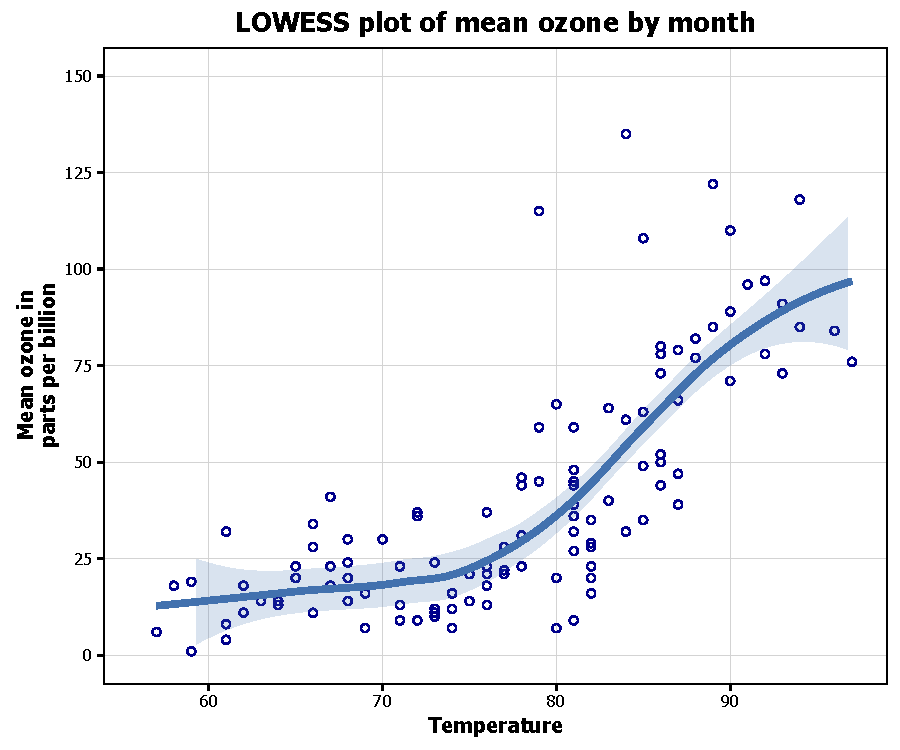
\includegraphics{12_Lowess_Plots_pdf/lowess_final-1} \end{center}

The first thing to do is load in the data and the libraries, as below.
We'll convert \texttt{Month} into a labelled factor in order to use it
as our grouping variable.

\begin{Shaded}
\begin{Highlighting}[]
\KeywordTok{library}\NormalTok{(datasets)}
\KeywordTok{library}\NormalTok{(ggplot2)}
\KeywordTok{library}\NormalTok{(ggthemes)}
\KeywordTok{library}\NormalTok{(grid)}
\KeywordTok{library}\NormalTok{(RColorBrewer)}

\KeywordTok{data}\NormalTok{(airquality)}
\end{Highlighting}
\end{Shaded}

\section{Creating a basic LOWESS plot, and what it can tell us about our
data}\label{creating-a-basic-lowess-plot-and-what-it-can-tell-us-about-our-data}

In order to initialise a plot we tell ggplot that \texttt{airquality} is
our data, and specify that our x-axis plots the \texttt{Temp} variable
and our y-axis plots the \texttt{Ozone} variable. We then instruct
ggplot to render this as a LOWESS curve by adding the
\texttt{stat\_smooth(method\ =\ "loess")} option. Note that the default
for \texttt{stat\_smooth} is to include the confidence interval.

\begin{Shaded}
\begin{Highlighting}[]
\NormalTok{p12 <-}\StringTok{ }\KeywordTok{ggplot}\NormalTok{(airquality, }\KeywordTok{aes}\NormalTok{(}\DataTypeTok{x =} \NormalTok{Temp, }\DataTypeTok{y =} \NormalTok{Ozone)) +}\StringTok{ }
\StringTok{  }\KeywordTok{geom_point}\NormalTok{() +}\StringTok{ }
\StringTok{  }\KeywordTok{stat_smooth}\NormalTok{(}\DataTypeTok{method =} \StringTok{"loess"}\NormalTok{)}
\NormalTok{p12}
\end{Highlighting}
\end{Shaded}

\begin{center}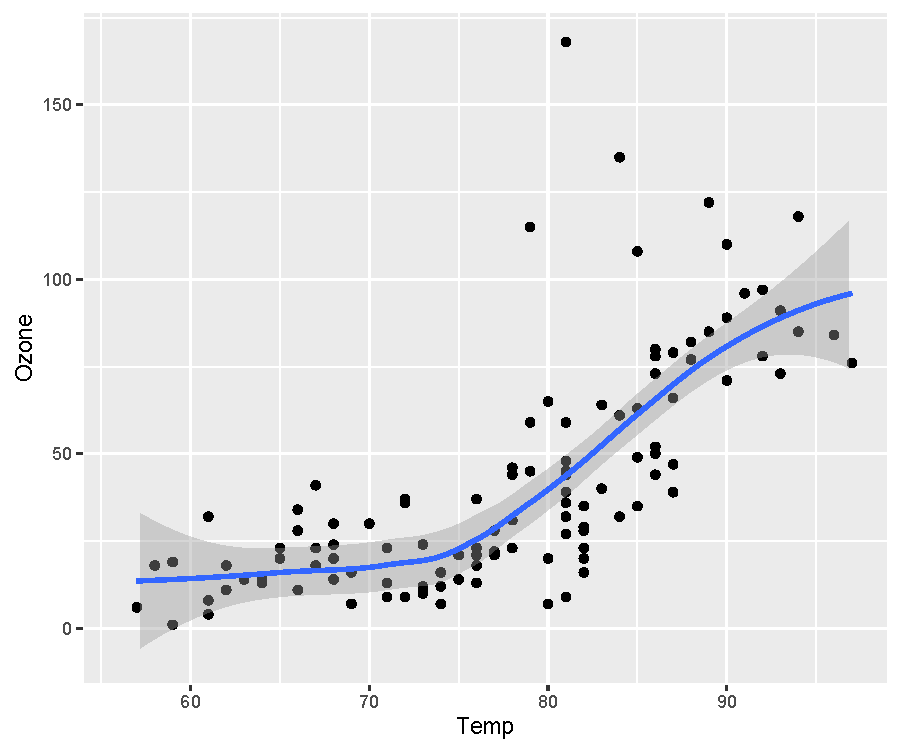
\includegraphics{12_Lowess_Plots_pdf/lowess_1-1} \end{center}

We can see that while the relationship between \texttt{Temp} and
\texttt{Ozone} is fairly linear, the LOWESS plot is demonstrating there
may be a threshold effect where ozone only starts increasing as
temperatures pass around 75 degrees Fahrenheit. To assess whether this
is the case, let's see how a standard linear fit between these variables
looks.

\begin{Shaded}
\begin{Highlighting}[]
\NormalTok{p12 <-}\StringTok{ }\KeywordTok{ggplot}\NormalTok{(airquality, }\KeywordTok{aes}\NormalTok{(}\DataTypeTok{x =} \NormalTok{Temp, }\DataTypeTok{y =} \NormalTok{Ozone)) +}\StringTok{ }
\StringTok{  }\KeywordTok{geom_point}\NormalTok{() +}\StringTok{ }
\StringTok{  }\KeywordTok{geom_smooth}\NormalTok{(}\DataTypeTok{method=}\NormalTok{lm)}
\NormalTok{p12}
\end{Highlighting}
\end{Shaded}

\begin{center}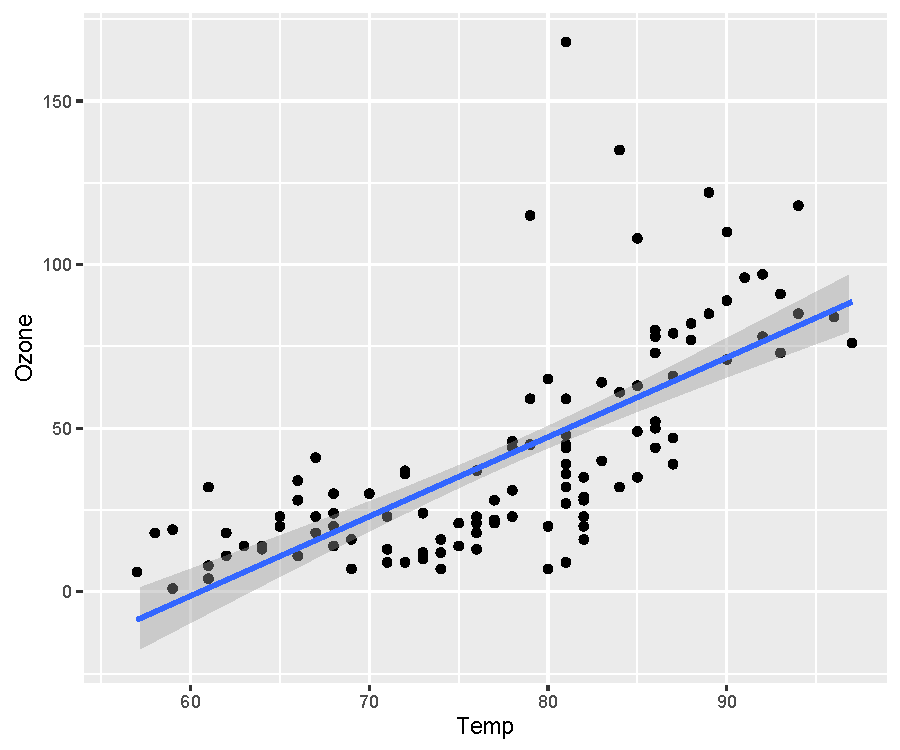
\includegraphics{12_Lowess_Plots_pdf/lowess_2-1} \end{center}

Let's now have a look at the amount of variance it explains in ozone
levels by extracting the adjusted \(R^2\) from the linear regression
model between these two variables.

\begin{Shaded}
\begin{Highlighting}[]
\NormalTok{m1 <-}\StringTok{ }\KeywordTok{summary}\NormalTok{(}\KeywordTok{lm}\NormalTok{(Ozone ~}\StringTok{ }\NormalTok{Temp, }\DataTypeTok{data =} \NormalTok{airquality))}
\NormalTok{m1$adj.r.squared}
\end{Highlighting}
\end{Shaded}

\begin{verbatim}
[1] 0.4832134
\end{verbatim}

You can see that the line comes away from the data at several points,
which will have increased the error in the regression model and brought
down the overall \(R^2\). Let's see whether we can get a better result
by fitting a quadratic model.

\begin{Shaded}
\begin{Highlighting}[]
\NormalTok{p12 <-}\StringTok{ }\KeywordTok{ggplot}\NormalTok{(airquality, }\KeywordTok{aes}\NormalTok{(}\DataTypeTok{x =} \NormalTok{Temp, }\DataTypeTok{y =} \NormalTok{Ozone)) +}\StringTok{ }
\StringTok{  }\KeywordTok{geom_point}\NormalTok{(}\DataTypeTok{shape=}\DecValTok{1}\NormalTok{) +}\StringTok{ }
\StringTok{  }\KeywordTok{stat_smooth}\NormalTok{(}\DataTypeTok{method =} \StringTok{"lm"}\NormalTok{, }\DataTypeTok{formula =} \NormalTok{y ~}\StringTok{ }\NormalTok{x +}\StringTok{ }\KeywordTok{I}\NormalTok{(x^}\DecValTok{2}\NormalTok{))}
\NormalTok{p12}
\end{Highlighting}
\end{Shaded}

\begin{center}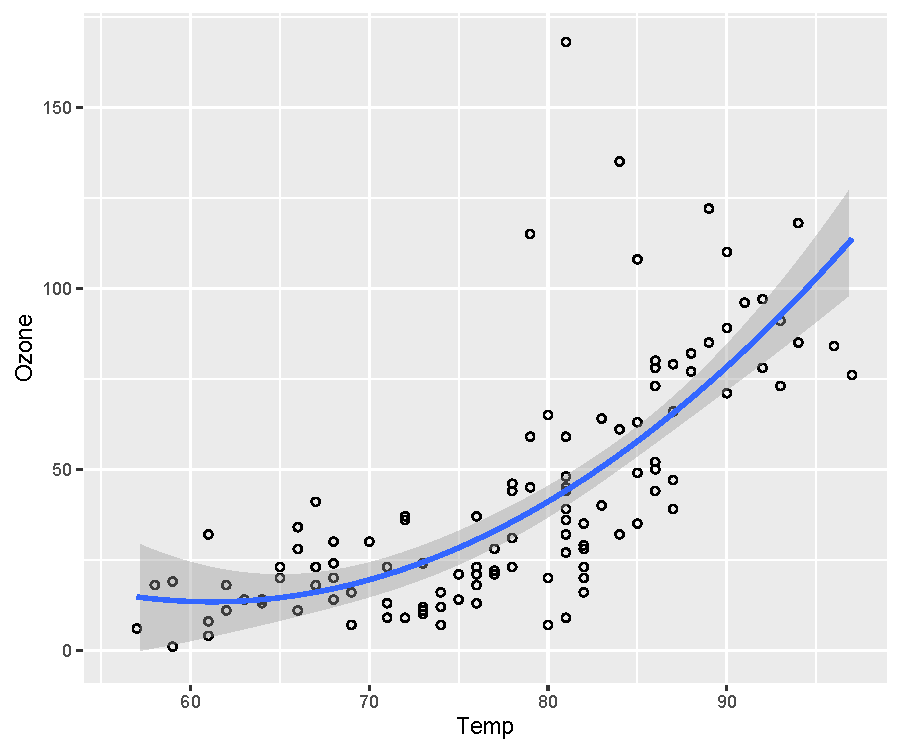
\includegraphics{12_Lowess_Plots_pdf/lowess_3-1} \end{center}

You can see this fits the data \emph{much} better. Let's see if the
regression model confirms this:

\begin{Shaded}
\begin{Highlighting}[]
\NormalTok{m2 <-}\StringTok{ }\KeywordTok{summary}\NormalTok{(}\KeywordTok{lm}\NormalTok{(Ozone ~}\StringTok{ }\NormalTok{Temp +}\StringTok{ }\KeywordTok{I}\NormalTok{(Temp^}\DecValTok{2}\NormalTok{), }\DataTypeTok{data =} \NormalTok{airquality))}
\NormalTok{m2$adj.r.squared}
\end{Highlighting}
\end{Shaded}

\begin{verbatim}
[1] 0.5361501
\end{verbatim}

You can see that we've managed to explain an additional 5\% of variance
in ozone levels by fitting a quadratic model rather than defaulting to a
linear model. Using LOWESS plots to explore the relationships between
your variables can therefore guide you in choosing the the right
regression model in a fairly pain-free way.

\section{Changing the width of the
bins}\label{changing-the-width-of-the-bins}

An important part of fitting LOWESS curves is that you can change the
number of bins that the x-axis is divided into by using the argument
\texttt{n}. More bins smooth out the line more, while less make it
closer to linear. The default number is 80, and here we will change it
to 5 so you can see the difference.

\begin{Shaded}
\begin{Highlighting}[]
\NormalTok{p12 <-}\StringTok{ }\KeywordTok{ggplot}\NormalTok{(airquality, }\KeywordTok{aes}\NormalTok{(}\DataTypeTok{x =} \NormalTok{Temp, }\DataTypeTok{y =} \NormalTok{Ozone)) +}\StringTok{ }
\StringTok{  }\KeywordTok{geom_point}\NormalTok{() +}\StringTok{ }
\StringTok{  }\KeywordTok{geom_smooth}\NormalTok{(}\DataTypeTok{method =} \StringTok{"loess"}\NormalTok{, }\DataTypeTok{n =} \DecValTok{5}\NormalTok{)}
\NormalTok{p12}
\end{Highlighting}
\end{Shaded}

\begin{center}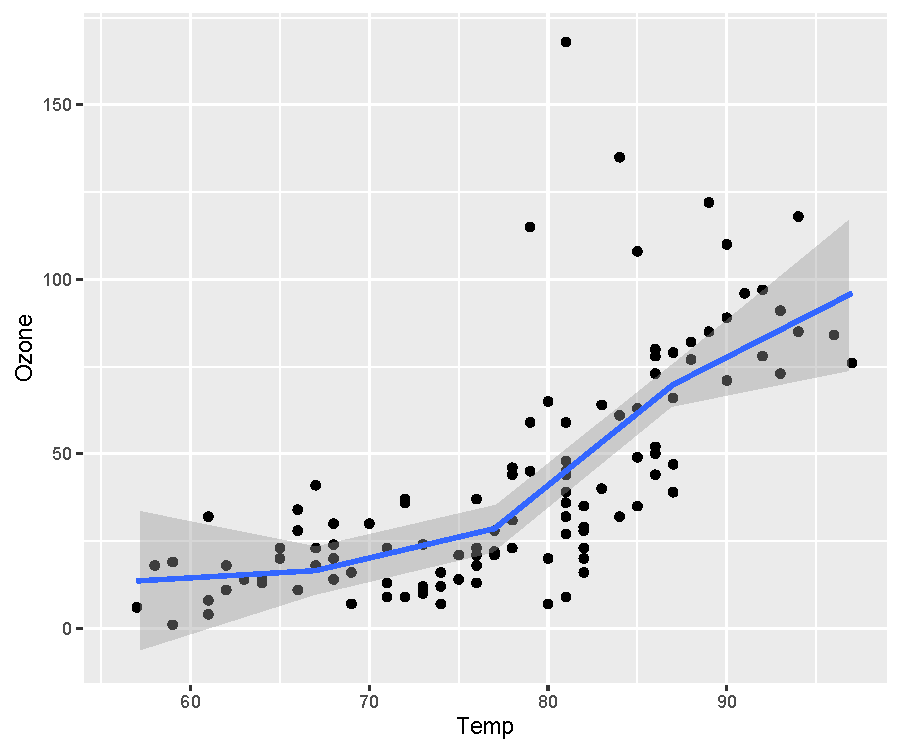
\includegraphics{12_Lowess_Plots_pdf/lowess_4-1} \end{center}

\section{Customising axis labels}\label{customising-axis-labels}

Now that we've established the rationale for using them, let's get down
to customising our basic LOWESS plot.

In order to change the axis labels, we have a couple of options. In this
case, we have used the \texttt{scale\_x\_continuous} and
\texttt{scale\_y\_continuous} options, as these have further
customisation options for the axes we will use below. In each, we add
the desired name to the \texttt{name} argument as a string.

\begin{Shaded}
\begin{Highlighting}[]
\NormalTok{p12 <-}\StringTok{ }\KeywordTok{ggplot}\NormalTok{(airquality, }\KeywordTok{aes}\NormalTok{(}\DataTypeTok{x =} \NormalTok{Temp, }\DataTypeTok{y =} \NormalTok{Ozone)) +}\StringTok{ }
\StringTok{  }\KeywordTok{geom_point}\NormalTok{() +}\StringTok{ }
\StringTok{  }\KeywordTok{stat_smooth}\NormalTok{(}\DataTypeTok{method =} \StringTok{"loess"}\NormalTok{) +}
\StringTok{  }\KeywordTok{scale_x_continuous}\NormalTok{(}\DataTypeTok{name =} \StringTok{"Temperature"}\NormalTok{) +}
\StringTok{  }\KeywordTok{scale_y_continuous}\NormalTok{(}\DataTypeTok{name =} \StringTok{"Mean ozone in parts per billion"}\NormalTok{)}
\NormalTok{p12}
\end{Highlighting}
\end{Shaded}

\begin{center}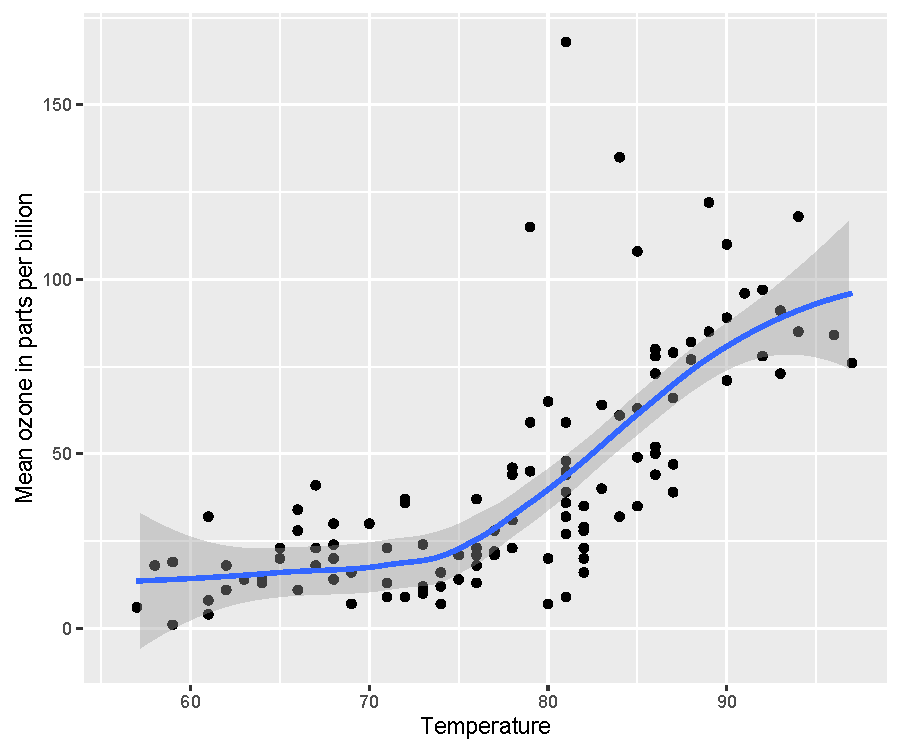
\includegraphics{12_Lowess_Plots_pdf/lowess_5-1} \end{center}

ggplot also allows for the use of multiline names (in both axes and
titles). Here, we've changed the y-axis label so that it goes over two
lines using the \texttt{\textbackslash{}n} character to break the line.

\begin{Shaded}
\begin{Highlighting}[]
\NormalTok{p12 <-}\StringTok{ }\NormalTok{p12 +}\StringTok{ }\KeywordTok{scale_y_continuous}\NormalTok{(}\DataTypeTok{name =} \StringTok{"Mean ozone in}\CharTok{\textbackslash{}n}\StringTok{parts per billion"}\NormalTok{)}
\NormalTok{p12}
\end{Highlighting}
\end{Shaded}

\begin{center}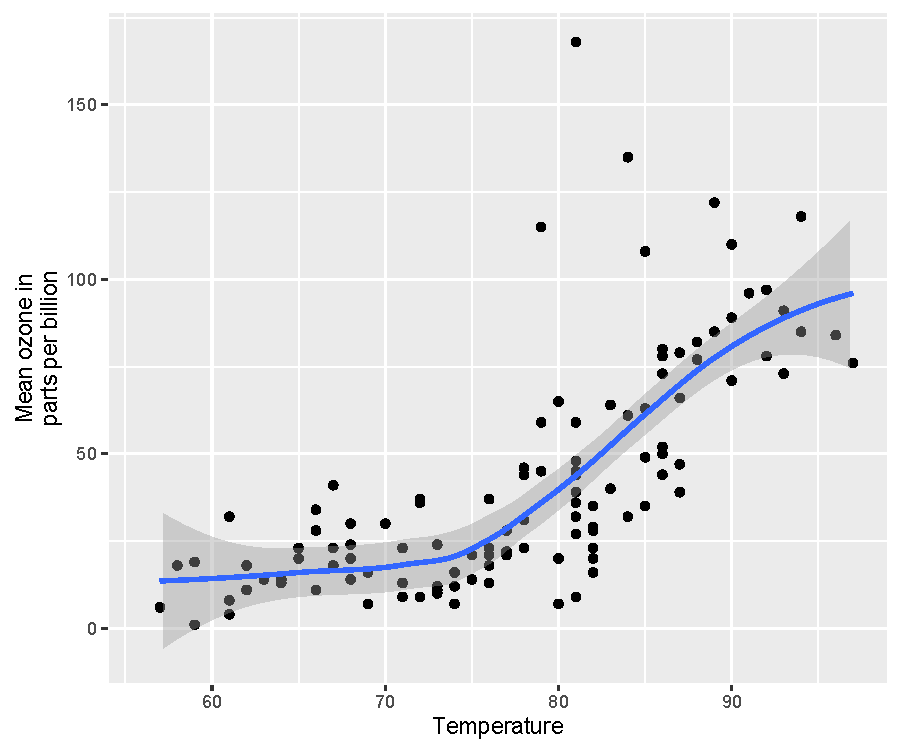
\includegraphics{12_Lowess_Plots_pdf/lowess_6-1} \end{center}

\section{Changing axis ticks}\label{changing-axis-ticks}

The next thing we will change is the axis ticks. Let's make the y-axis
ticks appear at every 25 units rather than 50 using the
\texttt{breaks\ =\ seq(0,\ 150,\ 25)} argument in
\texttt{scale\_y\_continuous}. (The \texttt{seq} function is a base R
function that indicates the start and endpoints and the units to
increment by respectively. See \texttt{help(seq)} for more information.)
We ensure that the y-axis begins and ends where we want by also adding
the argument \texttt{limits\ =\ c(0,\ 150)} to
\texttt{scale\_y\_continuous}.

\begin{Shaded}
\begin{Highlighting}[]
\NormalTok{p12 <-}\StringTok{ }\NormalTok{p12 +}\StringTok{ }\KeywordTok{scale_y_continuous}\NormalTok{(}\DataTypeTok{name =} \StringTok{"Mean ozone in}\CharTok{\textbackslash{}n}\StringTok{parts per billion"}\NormalTok{,}
                                \DataTypeTok{breaks =} \KeywordTok{seq}\NormalTok{(}\DecValTok{0}\NormalTok{, }\DecValTok{150}\NormalTok{, }\DecValTok{25}\NormalTok{), }\DataTypeTok{limits=}\KeywordTok{c}\NormalTok{(}\DecValTok{0}\NormalTok{, }\DecValTok{150}\NormalTok{))}
\NormalTok{p12}
\end{Highlighting}
\end{Shaded}

\begin{center}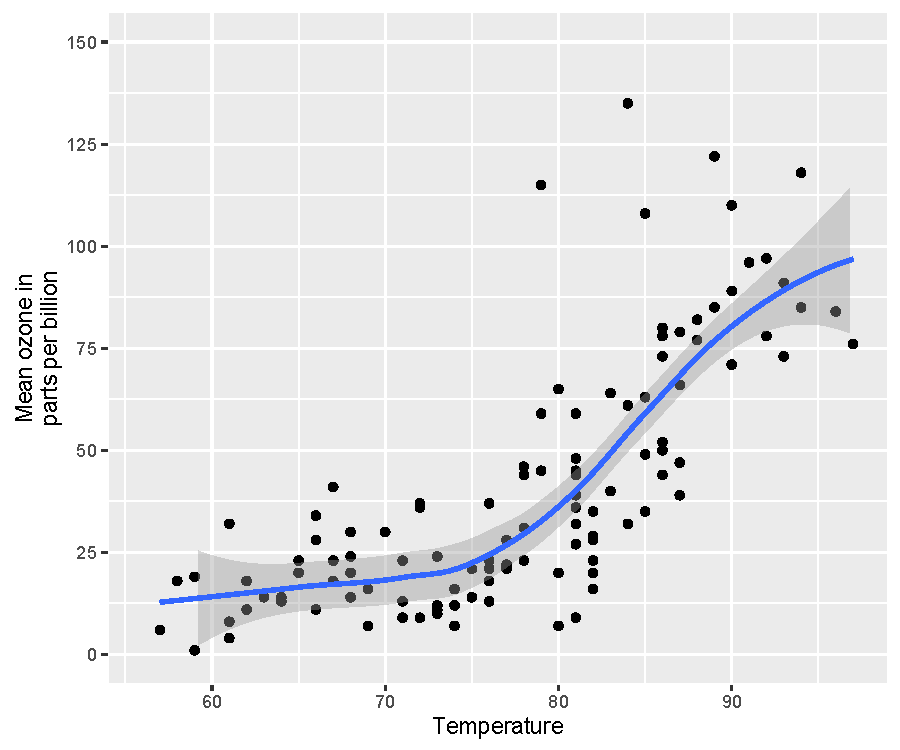
\includegraphics{12_Lowess_Plots_pdf/lowess_7-1} \end{center}

\section{Adding a title}\label{adding-a-title}

To add a title, we include the option \texttt{ggtitle} and include the
name of the graph as a string argument.

\begin{Shaded}
\begin{Highlighting}[]
\NormalTok{p12 <-}\StringTok{ }\NormalTok{p12 +}\StringTok{ }\KeywordTok{ggtitle}\NormalTok{(}\StringTok{"LOWESS plot of mean ozone by month"}\NormalTok{)}
\NormalTok{p12}
\end{Highlighting}
\end{Shaded}

\begin{center}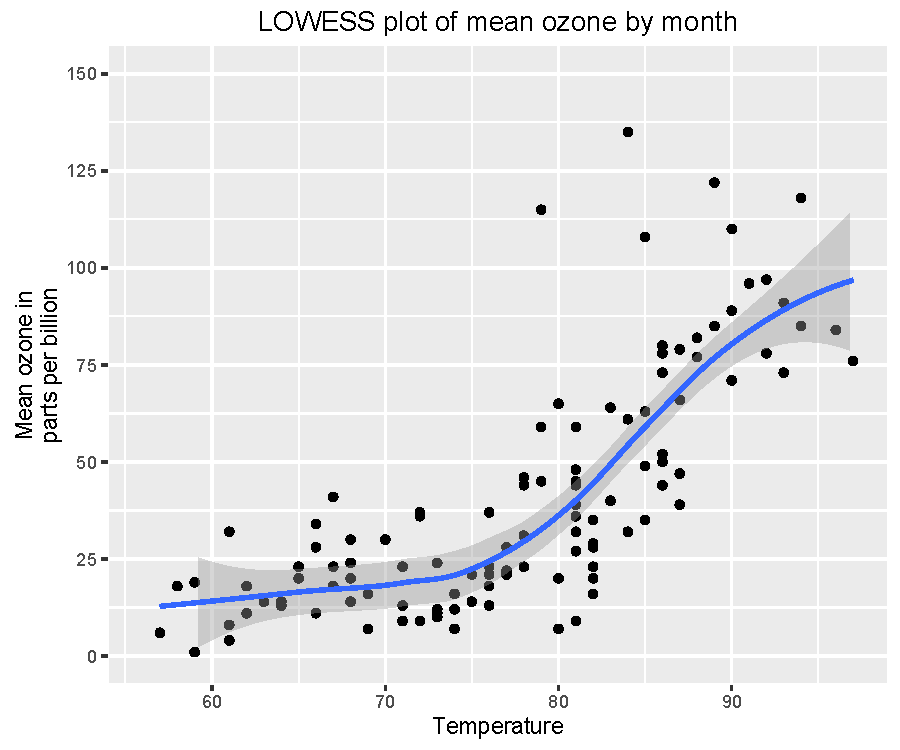
\includegraphics{12_Lowess_Plots_pdf/lowess_8-1} \end{center}

\section{Changing the colour and size of the LOWESS
curve}\label{changing-the-colour-and-size-of-the-lowess-curve}

To change the colour of the LOWESS curve, we add a valid colour to the
\texttt{colour} argument in \texttt{geom\_smooth()} (note that we
assigned this colour to a variable outside of the plot to make it easier
to change it). A list of valid colours is
\href{http://www.stat.columbia.edu/~tzheng/files/Rcolor.pdf}{here}.

\begin{Shaded}
\begin{Highlighting}[]
\NormalTok{fill <-}\StringTok{ "gold1"}

\NormalTok{p12 <-}\StringTok{ }\KeywordTok{ggplot}\NormalTok{(airquality, }\KeywordTok{aes}\NormalTok{(}\DataTypeTok{x =} \NormalTok{Temp, }\DataTypeTok{y =} \NormalTok{Ozone)) +}\StringTok{ }
\StringTok{  }\KeywordTok{geom_point}\NormalTok{() +}\StringTok{ }
\StringTok{  }\KeywordTok{geom_smooth}\NormalTok{(}\DataTypeTok{method =} \StringTok{"loess"}\NormalTok{, }\DataTypeTok{colour =} \NormalTok{fill) +}
\StringTok{  }\KeywordTok{scale_x_continuous}\NormalTok{(}\DataTypeTok{name =} \StringTok{"Temperature"}\NormalTok{) +}
\StringTok{  }\KeywordTok{scale_y_continuous}\NormalTok{(}\DataTypeTok{name =} \StringTok{"Mean ozone in}\CharTok{\textbackslash{}n}\StringTok{parts per billion"}\NormalTok{,}
                     \DataTypeTok{breaks =} \KeywordTok{seq}\NormalTok{(}\DecValTok{0}\NormalTok{, }\DecValTok{150}\NormalTok{, }\DecValTok{25}\NormalTok{), }\DataTypeTok{limits=}\KeywordTok{c}\NormalTok{(}\DecValTok{0}\NormalTok{, }\DecValTok{150}\NormalTok{)) +}
\StringTok{  }\KeywordTok{ggtitle}\NormalTok{(}\StringTok{"LOWESS plot of mean ozone by month"}\NormalTok{)}
\NormalTok{p12}
\end{Highlighting}
\end{Shaded}

\begin{center}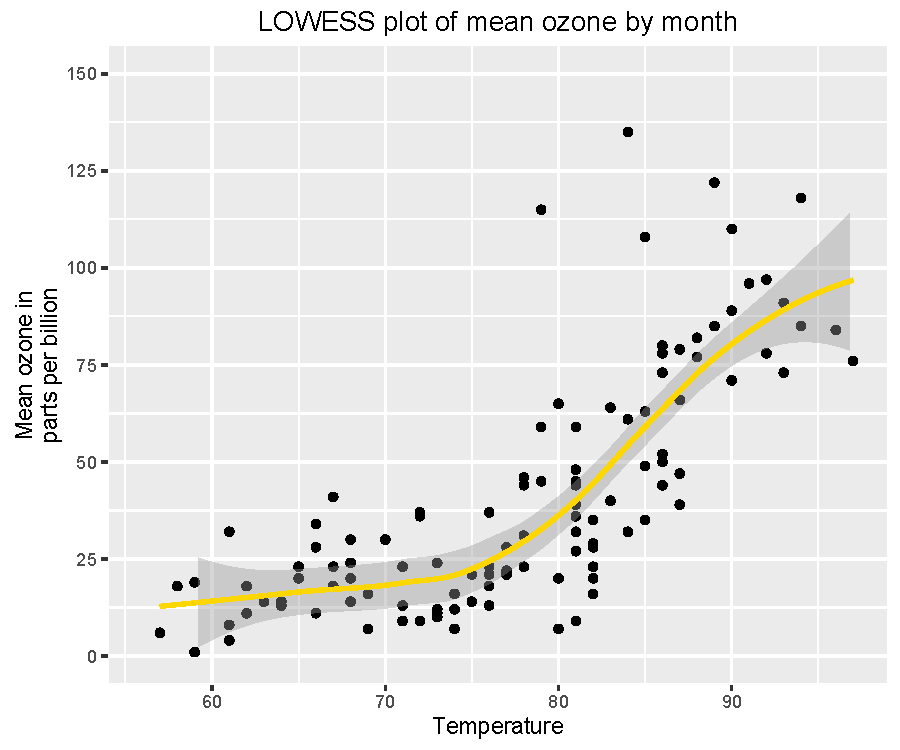
\includegraphics{12_Lowess_Plots_pdf/lowess_9-1} \end{center}

If you want to go beyond the options in the list above, you can also
specify exact HEX colours by including them as a string preceded by a
hash, e.g., ``\#FFFFFF''. Below, we have called a shade of blue for the
line using its HEX code.

\begin{Shaded}
\begin{Highlighting}[]
\NormalTok{fill <-}\StringTok{ "#4271AE"}

\NormalTok{p12 <-}\StringTok{ }\KeywordTok{ggplot}\NormalTok{(airquality, }\KeywordTok{aes}\NormalTok{(}\DataTypeTok{x =} \NormalTok{Temp, }\DataTypeTok{y =} \NormalTok{Ozone)) +}\StringTok{ }
\StringTok{  }\KeywordTok{geom_point}\NormalTok{() +}\StringTok{ }
\StringTok{  }\KeywordTok{geom_smooth}\NormalTok{(}\DataTypeTok{method =} \StringTok{"loess"}\NormalTok{, }\DataTypeTok{colour =} \NormalTok{fill) +}
\StringTok{  }\KeywordTok{scale_x_continuous}\NormalTok{(}\DataTypeTok{name =} \StringTok{"Temperature"}\NormalTok{) +}
\StringTok{  }\KeywordTok{scale_y_continuous}\NormalTok{(}\DataTypeTok{name =} \StringTok{"Mean ozone in}\CharTok{\textbackslash{}n}\StringTok{parts per billion"}\NormalTok{,}
                     \DataTypeTok{breaks =} \KeywordTok{seq}\NormalTok{(}\DecValTok{0}\NormalTok{, }\DecValTok{150}\NormalTok{, }\DecValTok{25}\NormalTok{), }\DataTypeTok{limits=}\KeywordTok{c}\NormalTok{(}\DecValTok{0}\NormalTok{, }\DecValTok{150}\NormalTok{)) +}
\StringTok{  }\KeywordTok{ggtitle}\NormalTok{(}\StringTok{"LOWESS plot of mean ozone by month"}\NormalTok{)}
\NormalTok{p12}
\end{Highlighting}
\end{Shaded}

\begin{center}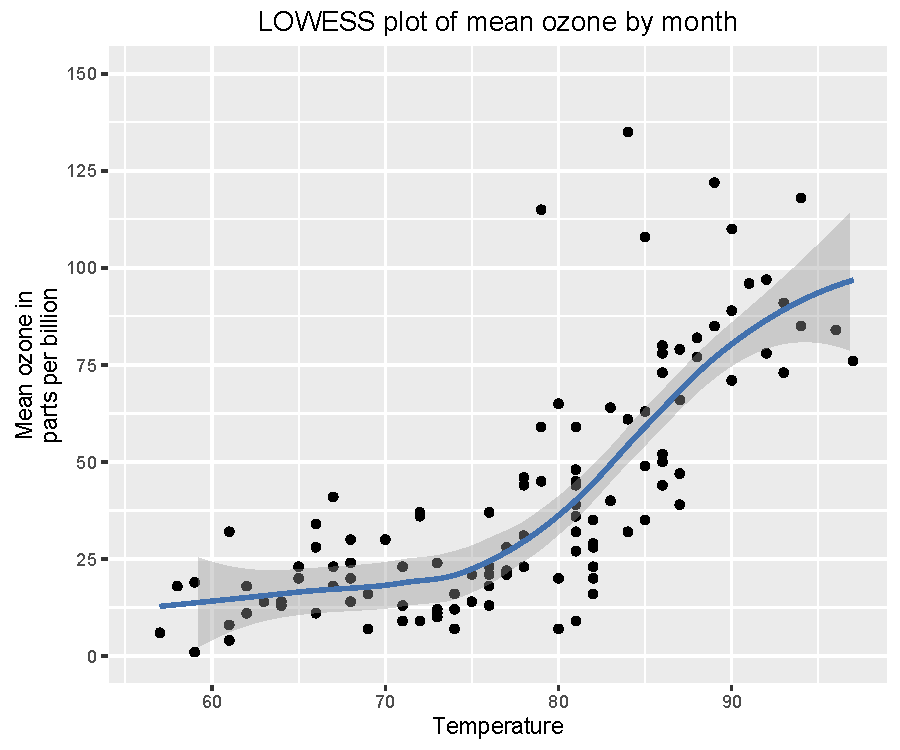
\includegraphics{12_Lowess_Plots_pdf/lowess_10-1} \end{center}

We can also increase the thickness of the line using the \texttt{size}
option in \texttt{geom\_smooth()}.

\begin{Shaded}
\begin{Highlighting}[]
\NormalTok{fill <-}\StringTok{ "#4271AE"}

\NormalTok{p12 <-}\StringTok{ }\KeywordTok{ggplot}\NormalTok{(airquality, }\KeywordTok{aes}\NormalTok{(}\DataTypeTok{x =} \NormalTok{Temp, }\DataTypeTok{y =} \NormalTok{Ozone)) +}\StringTok{ }
\StringTok{  }\KeywordTok{geom_point}\NormalTok{() +}\StringTok{ }
\StringTok{  }\KeywordTok{geom_smooth}\NormalTok{(}\DataTypeTok{method =} \StringTok{"loess"}\NormalTok{, }\DataTypeTok{colour =} \NormalTok{fill, }\DataTypeTok{size =} \FloatTok{1.5}\NormalTok{) +}
\StringTok{  }\KeywordTok{scale_x_continuous}\NormalTok{(}\DataTypeTok{name =} \StringTok{"Temperature"}\NormalTok{) +}
\StringTok{  }\KeywordTok{scale_y_continuous}\NormalTok{(}\DataTypeTok{name =} \StringTok{"Mean ozone in}\CharTok{\textbackslash{}n}\StringTok{parts per billion"}\NormalTok{,}
                     \DataTypeTok{breaks =} \KeywordTok{seq}\NormalTok{(}\DecValTok{0}\NormalTok{, }\DecValTok{150}\NormalTok{, }\DecValTok{25}\NormalTok{), }\DataTypeTok{limits=}\KeywordTok{c}\NormalTok{(}\DecValTok{0}\NormalTok{, }\DecValTok{150}\NormalTok{)) +}
\StringTok{  }\KeywordTok{ggtitle}\NormalTok{(}\StringTok{"LOWESS plot of mean ozone by month"}\NormalTok{)}
\NormalTok{p12}
\end{Highlighting}
\end{Shaded}

\begin{center}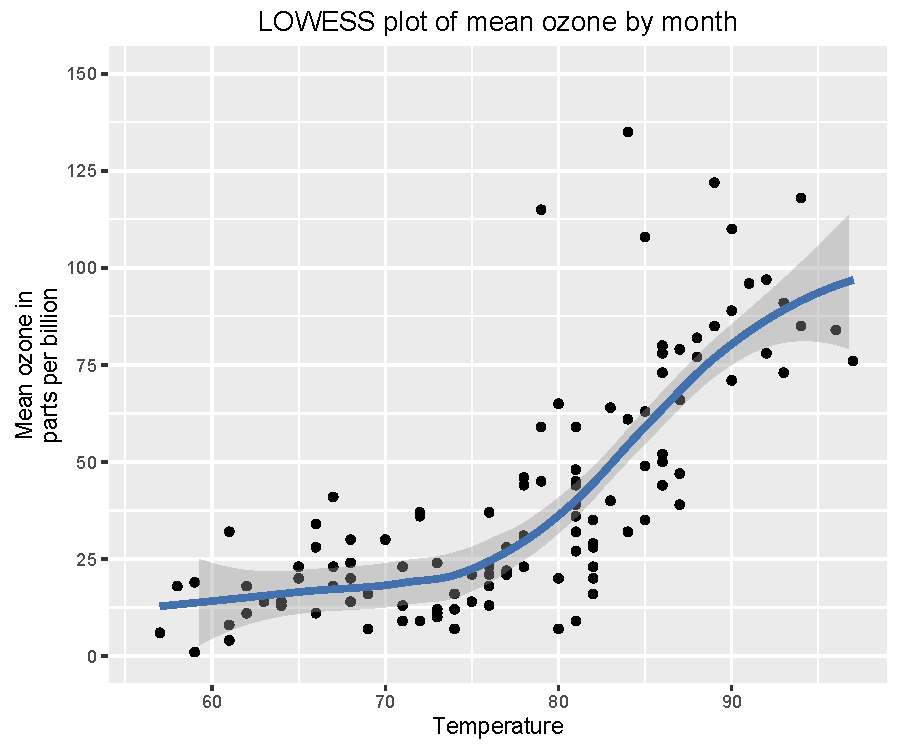
\includegraphics{12_Lowess_Plots_pdf/lowess_11-1} \end{center}

\section{Changing the appearance of the confidence
interval}\label{changing-the-appearance-of-the-confidence-interval}

We can also alter how the confidence interval around the LOWESS curve
looks. We can change the transparency using the argument \texttt{alpha}
in \texttt{geom\_smooth()}. This ranges from 0 to 1. Here we will
increase the transparency of the confidence interval.

\begin{Shaded}
\begin{Highlighting}[]
\NormalTok{fill <-}\StringTok{ "#4271AE"}

\NormalTok{p12 <-}\StringTok{ }\KeywordTok{ggplot}\NormalTok{(airquality, }\KeywordTok{aes}\NormalTok{(}\DataTypeTok{x =} \NormalTok{Temp, }\DataTypeTok{y =} \NormalTok{Ozone)) +}\StringTok{ }
\StringTok{  }\KeywordTok{geom_point}\NormalTok{() +}\StringTok{ }
\StringTok{  }\KeywordTok{geom_smooth}\NormalTok{(}\DataTypeTok{method =} \StringTok{"loess"}\NormalTok{, }\DataTypeTok{colour =} \NormalTok{fill, }\DataTypeTok{size =} \FloatTok{1.5}\NormalTok{, }\DataTypeTok{alpha =} \FloatTok{0.2}\NormalTok{) +}
\StringTok{  }\KeywordTok{scale_x_continuous}\NormalTok{(}\DataTypeTok{name =} \StringTok{"Temperature"}\NormalTok{) +}
\StringTok{  }\KeywordTok{scale_y_continuous}\NormalTok{(}\DataTypeTok{name =} \StringTok{"Mean ozone in}\CharTok{\textbackslash{}n}\StringTok{parts per billion"}\NormalTok{,}
                     \DataTypeTok{breaks =} \KeywordTok{seq}\NormalTok{(}\DecValTok{0}\NormalTok{, }\DecValTok{150}\NormalTok{, }\DecValTok{25}\NormalTok{), }\DataTypeTok{limits=}\KeywordTok{c}\NormalTok{(}\DecValTok{0}\NormalTok{, }\DecValTok{150}\NormalTok{)) +}
\StringTok{  }\KeywordTok{ggtitle}\NormalTok{(}\StringTok{"LOWESS plot of mean ozone by month"}\NormalTok{)}
\NormalTok{p12}
\end{Highlighting}
\end{Shaded}

\begin{center}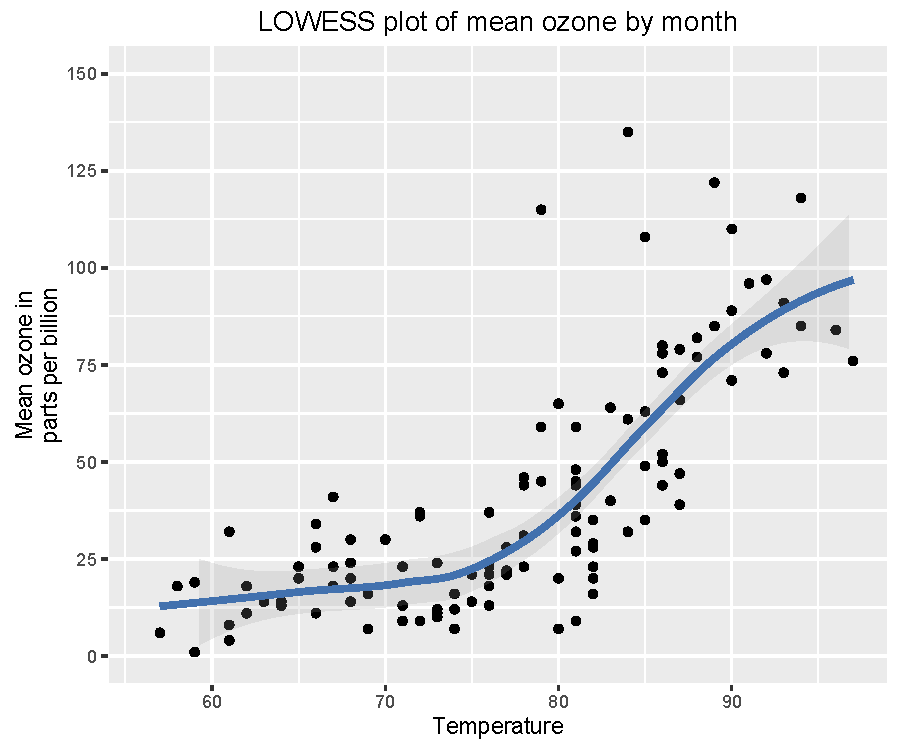
\includegraphics{12_Lowess_Plots_pdf/lowess_12-1} \end{center}

We can also change the colour of the confidence interval from the
default grey using the argument \texttt{fill}, also within
\texttt{geom\_smooth()}. Let's change it to the same blue as our LOWESS
curve.

\begin{Shaded}
\begin{Highlighting}[]
\NormalTok{fill <-}\StringTok{ "#4271AE"}

\NormalTok{p12 <-}\StringTok{ }\KeywordTok{ggplot}\NormalTok{(airquality, }\KeywordTok{aes}\NormalTok{(}\DataTypeTok{x =} \NormalTok{Temp, }\DataTypeTok{y =} \NormalTok{Ozone)) +}\StringTok{ }
\StringTok{  }\KeywordTok{geom_point}\NormalTok{() +}\StringTok{ }
\StringTok{  }\KeywordTok{geom_smooth}\NormalTok{(}\DataTypeTok{method =} \StringTok{"loess"}\NormalTok{, }\DataTypeTok{colour =} \NormalTok{fill, }\DataTypeTok{size =} \FloatTok{1.5}\NormalTok{, }
              \DataTypeTok{alpha =} \FloatTok{0.2}\NormalTok{, }\DataTypeTok{fill =} \NormalTok{fill) +}
\StringTok{  }\KeywordTok{scale_x_continuous}\NormalTok{(}\DataTypeTok{name =} \StringTok{"Temperature"}\NormalTok{) +}
\StringTok{  }\KeywordTok{scale_y_continuous}\NormalTok{(}\DataTypeTok{name =} \StringTok{"Mean ozone in}\CharTok{\textbackslash{}n}\StringTok{parts per billion"}\NormalTok{,}
                     \DataTypeTok{breaks =} \KeywordTok{seq}\NormalTok{(}\DecValTok{0}\NormalTok{, }\DecValTok{150}\NormalTok{, }\DecValTok{25}\NormalTok{), }\DataTypeTok{limits=}\KeywordTok{c}\NormalTok{(}\DecValTok{0}\NormalTok{, }\DecValTok{150}\NormalTok{)) +}
\StringTok{  }\KeywordTok{ggtitle}\NormalTok{(}\StringTok{"LOWESS plot of mean ozone by month"}\NormalTok{)}
\NormalTok{p12}
\end{Highlighting}
\end{Shaded}

\begin{center}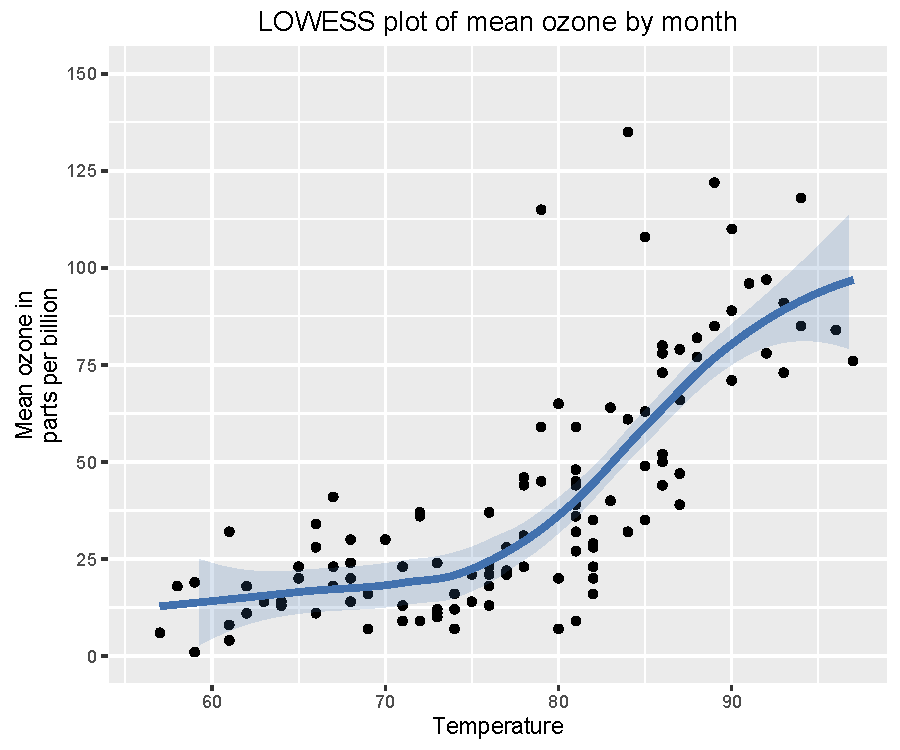
\includegraphics{12_Lowess_Plots_pdf/lowess_13-1} \end{center}

Finally, you can also turn off the confidence altogether by adding the
argument \texttt{se\ =\ FALSE} to \texttt{geom\_smooth()}.

\begin{Shaded}
\begin{Highlighting}[]
\NormalTok{fill <-}\StringTok{ "#4271AE"}

\NormalTok{p12 <-}\StringTok{ }\KeywordTok{ggplot}\NormalTok{(airquality, }\KeywordTok{aes}\NormalTok{(}\DataTypeTok{x =} \NormalTok{Temp, }\DataTypeTok{y =} \NormalTok{Ozone)) +}\StringTok{ }
\StringTok{  }\KeywordTok{geom_point}\NormalTok{() +}\StringTok{ }
\StringTok{  }\KeywordTok{geom_smooth}\NormalTok{(}\DataTypeTok{method =} \StringTok{"loess"}\NormalTok{, }\DataTypeTok{colour =} \NormalTok{fill, }\DataTypeTok{size =} \FloatTok{1.5}\NormalTok{, }\DataTypeTok{se =} \OtherTok{FALSE}\NormalTok{) +}
\StringTok{  }\KeywordTok{scale_x_continuous}\NormalTok{(}\DataTypeTok{name =} \StringTok{"Temperature"}\NormalTok{) +}
\StringTok{  }\KeywordTok{scale_y_continuous}\NormalTok{(}\DataTypeTok{name =} \StringTok{"Mean ozone in}\CharTok{\textbackslash{}n}\StringTok{parts per billion"}\NormalTok{,}
                     \DataTypeTok{breaks =} \KeywordTok{seq}\NormalTok{(}\DecValTok{0}\NormalTok{, }\DecValTok{150}\NormalTok{, }\DecValTok{25}\NormalTok{), }\DataTypeTok{limits=}\KeywordTok{c}\NormalTok{(}\DecValTok{0}\NormalTok{, }\DecValTok{150}\NormalTok{)) +}
\StringTok{  }\KeywordTok{ggtitle}\NormalTok{(}\StringTok{"LOWESS plot of mean ozone by month"}\NormalTok{)}
\NormalTok{p12}
\end{Highlighting}
\end{Shaded}

\begin{center}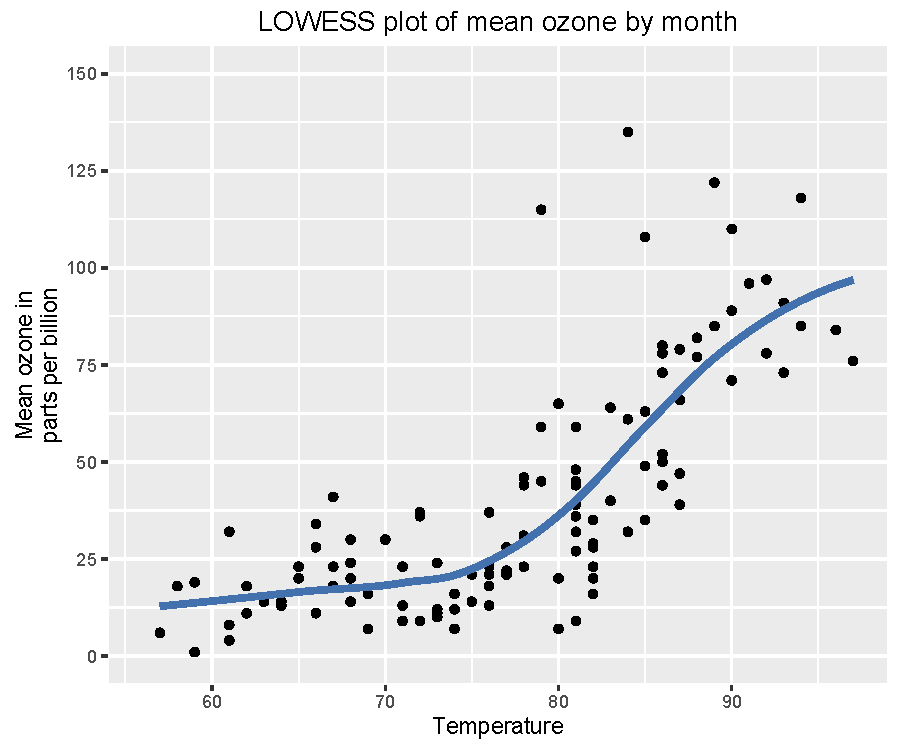
\includegraphics{12_Lowess_Plots_pdf/lowess_14-1} \end{center}

\section{Changing the appearance of the
scatterplot}\label{changing-the-appearance-of-the-scatterplot}

Of course, the LOWESS curve is not the only part of this plot. We can
also customise the appearance of the scatterplot underlying the curve.
Let's change the circles to shape 21, which is a circle that allows
different colours for the outline and fill, and change the colour of the
outline to dark blue. We can do this by adding the \texttt{shape} and
\texttt{colour} arguments to \texttt{geom\_point()} respectively.

\begin{Shaded}
\begin{Highlighting}[]
\NormalTok{fill <-}\StringTok{ "#4271AE"}

\NormalTok{p12 <-}\StringTok{ }\KeywordTok{ggplot}\NormalTok{(airquality, }\KeywordTok{aes}\NormalTok{(}\DataTypeTok{x =} \NormalTok{Temp, }\DataTypeTok{y =} \NormalTok{Ozone)) +}\StringTok{ }
\StringTok{  }\KeywordTok{geom_point}\NormalTok{(}\DataTypeTok{shape =} \DecValTok{21}\NormalTok{, }\DataTypeTok{colour =} \StringTok{"darkblue"}\NormalTok{) +}\StringTok{ }
\StringTok{  }\KeywordTok{geom_smooth}\NormalTok{(}\DataTypeTok{method =} \StringTok{"loess"}\NormalTok{, }\DataTypeTok{colour =} \NormalTok{fill, }\DataTypeTok{size =} \FloatTok{1.5}\NormalTok{, }
              \DataTypeTok{alpha =} \FloatTok{0.2}\NormalTok{, }\DataTypeTok{fill =} \NormalTok{fill) +}
\StringTok{  }\KeywordTok{scale_x_continuous}\NormalTok{(}\DataTypeTok{name =} \StringTok{"Temperature"}\NormalTok{) +}
\StringTok{  }\KeywordTok{scale_y_continuous}\NormalTok{(}\DataTypeTok{name =} \StringTok{"Mean ozone in}\CharTok{\textbackslash{}n}\StringTok{parts per billion"}\NormalTok{,}
                     \DataTypeTok{breaks =} \KeywordTok{seq}\NormalTok{(}\DecValTok{0}\NormalTok{, }\DecValTok{150}\NormalTok{, }\DecValTok{25}\NormalTok{), }\DataTypeTok{limits=}\KeywordTok{c}\NormalTok{(}\DecValTok{0}\NormalTok{, }\DecValTok{150}\NormalTok{)) +}
\StringTok{  }\KeywordTok{ggtitle}\NormalTok{(}\StringTok{"LOWESS plot of mean ozone by month"}\NormalTok{)}
\NormalTok{p12}
\end{Highlighting}
\end{Shaded}

\begin{center}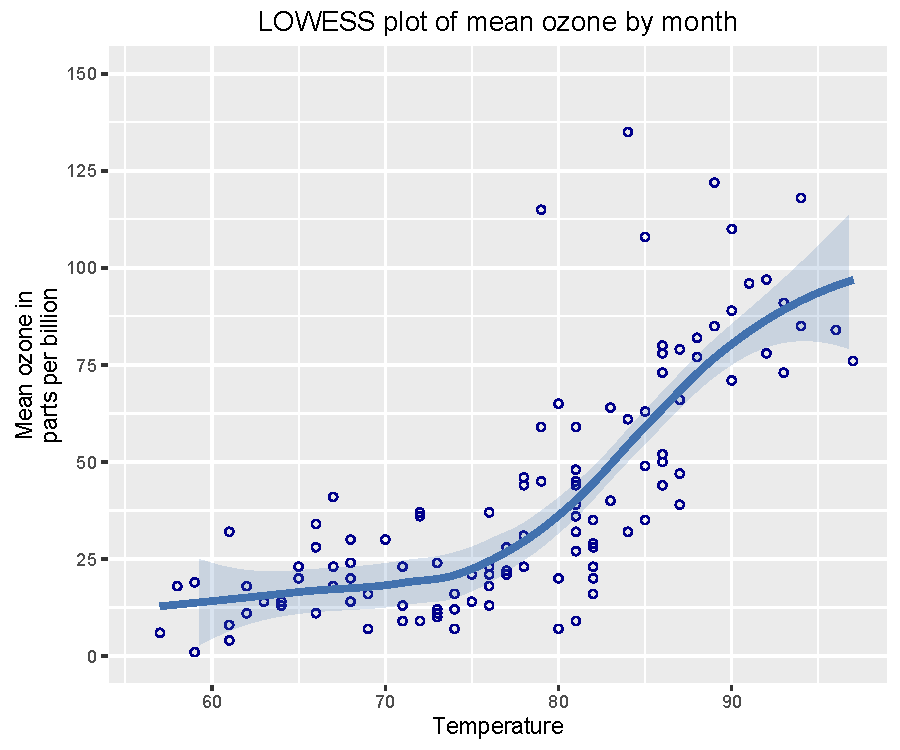
\includegraphics{12_Lowess_Plots_pdf/lowess_15-1} \end{center}

You can also get rid of the scatterplot points altogether by removing
the \texttt{geom\_point()} option. You can see we have also changed the
range of the y-axis in \texttt{scale\_y\_continuous()} so the graph sits
closer to the top of the LOWESS curve.

\begin{Shaded}
\begin{Highlighting}[]
\NormalTok{fill <-}\StringTok{ "#4271AE"}

\NormalTok{p12 <-}\StringTok{ }\KeywordTok{ggplot}\NormalTok{(airquality, }\KeywordTok{aes}\NormalTok{(}\DataTypeTok{x =} \NormalTok{Temp, }\DataTypeTok{y =} \NormalTok{Ozone)) +}\StringTok{ }
\StringTok{  }\KeywordTok{geom_smooth}\NormalTok{(}\DataTypeTok{method =} \StringTok{"loess"}\NormalTok{, }\DataTypeTok{colour =} \NormalTok{fill, }\DataTypeTok{size =} \FloatTok{1.5}\NormalTok{, }
              \DataTypeTok{alpha =} \FloatTok{0.2}\NormalTok{, }\DataTypeTok{fill =} \NormalTok{fill) +}
\StringTok{  }\KeywordTok{scale_x_continuous}\NormalTok{(}\DataTypeTok{name =} \StringTok{"Temperature"}\NormalTok{) +}
\StringTok{  }\KeywordTok{scale_y_continuous}\NormalTok{(}\DataTypeTok{name =} \StringTok{"Mean ozone in}\CharTok{\textbackslash{}n}\StringTok{parts per billion"}\NormalTok{,}
                     \DataTypeTok{breaks =} \KeywordTok{seq}\NormalTok{(}\DecValTok{0}\NormalTok{, }\DecValTok{125}\NormalTok{, }\DecValTok{25}\NormalTok{), }\DataTypeTok{limits=}\KeywordTok{c}\NormalTok{(}\DecValTok{0}\NormalTok{, }\DecValTok{125}\NormalTok{)) +}
\StringTok{  }\KeywordTok{ggtitle}\NormalTok{(}\StringTok{"LOWESS plot of mean ozone by month"}\NormalTok{)}
\NormalTok{p12}
\end{Highlighting}
\end{Shaded}

\begin{center}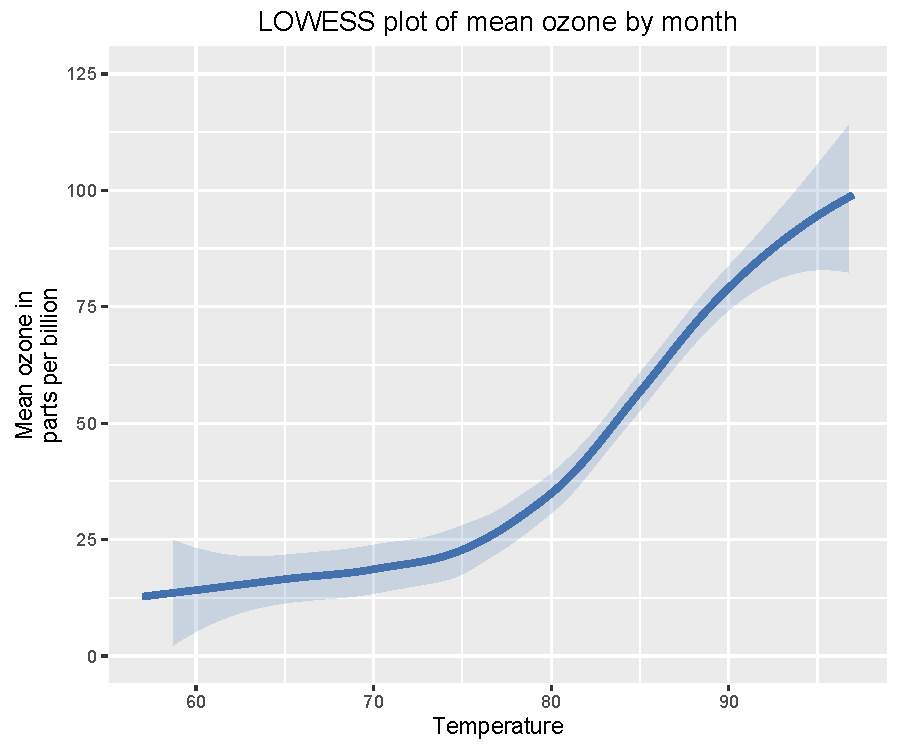
\includegraphics{12_Lowess_Plots_pdf/lowess_16-1} \end{center}

\section{Using the white theme}\label{using-the-white-theme}

As explained in the previous posts, we can also change the overall look
of the plot using themes. We'll start using a simple theme customisation
by adding \texttt{theme\_bw()}. As you can see, we can further tweak the
graph using the \texttt{theme} option, which we've used so far to change
the legend.

\begin{Shaded}
\begin{Highlighting}[]
\NormalTok{fill <-}\StringTok{ "#4271AE"}

\NormalTok{p12 <-}\StringTok{ }\KeywordTok{ggplot}\NormalTok{(airquality, }\KeywordTok{aes}\NormalTok{(}\DataTypeTok{x =} \NormalTok{Temp, }\DataTypeTok{y =} \NormalTok{Ozone)) +}\StringTok{ }
\StringTok{  }\KeywordTok{geom_point}\NormalTok{(}\DataTypeTok{shape =} \DecValTok{21}\NormalTok{, }\DataTypeTok{colour =} \StringTok{"darkblue"}\NormalTok{) +}\StringTok{ }
\StringTok{  }\KeywordTok{geom_smooth}\NormalTok{(}\DataTypeTok{method =} \StringTok{"loess"}\NormalTok{, }\DataTypeTok{colour =} \NormalTok{fill, }\DataTypeTok{size =} \FloatTok{1.5}\NormalTok{, }
              \DataTypeTok{alpha =} \FloatTok{0.2}\NormalTok{, }\DataTypeTok{fill =} \NormalTok{fill) +}
\StringTok{  }\KeywordTok{scale_x_continuous}\NormalTok{(}\DataTypeTok{name =} \StringTok{"Temperature"}\NormalTok{) +}
\StringTok{  }\KeywordTok{scale_y_continuous}\NormalTok{(}\DataTypeTok{name =} \StringTok{"Mean ozone in}\CharTok{\textbackslash{}n}\StringTok{parts per billion"}\NormalTok{,}
                     \DataTypeTok{breaks =} \KeywordTok{seq}\NormalTok{(}\DecValTok{0}\NormalTok{, }\DecValTok{150}\NormalTok{, }\DecValTok{25}\NormalTok{), }\DataTypeTok{limits=}\KeywordTok{c}\NormalTok{(}\DecValTok{0}\NormalTok{, }\DecValTok{150}\NormalTok{)) +}
\StringTok{  }\KeywordTok{ggtitle}\NormalTok{(}\StringTok{"LOWESS plot of mean ozone by month"}\NormalTok{) +}
\StringTok{  }\KeywordTok{theme_bw}\NormalTok{()}
\NormalTok{p12}
\end{Highlighting}
\end{Shaded}

\begin{center}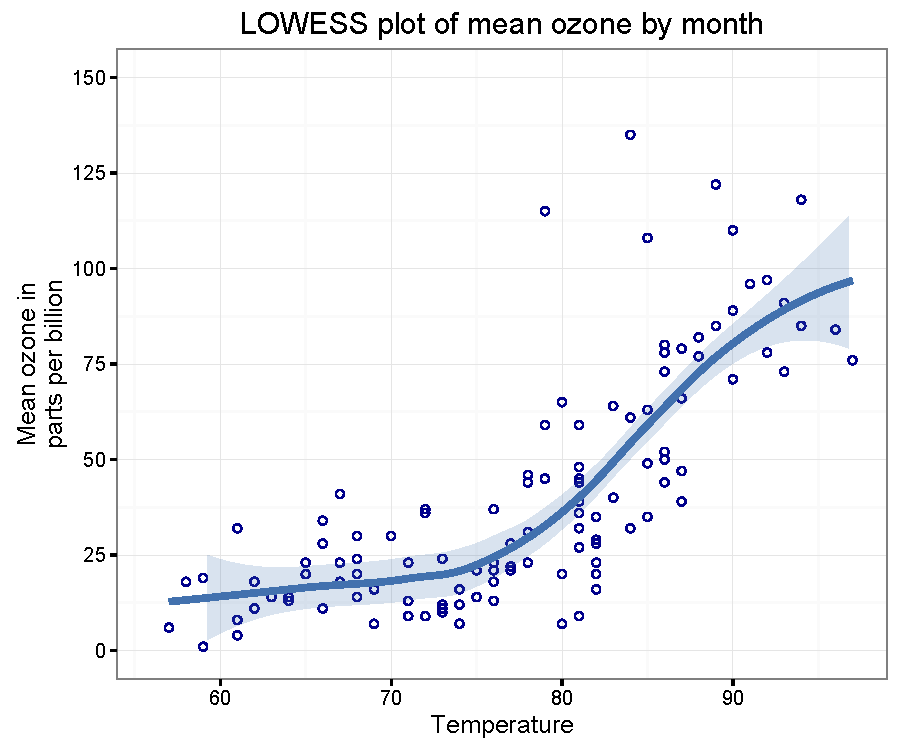
\includegraphics{12_Lowess_Plots_pdf/lowess_17-1} \end{center}

\section{Creating an XKCD style
chart}\label{creating-an-xkcd-style-chart}

Of course, you may want to create your own themes as well.
\texttt{ggplot2} allows for a very high degree of customisation,
including allowing you to use imported fonts. Below is an example of a
theme Mauricio was able to create which mimics the visual style of
\href{http://xkcd.com/}{XKCD}. In order to create this chart, you first
need to import the XKCD font, and load it into R using the
\texttt{extrafont} package.

\begin{Shaded}
\begin{Highlighting}[]
\NormalTok{p12 <-}\StringTok{ }\KeywordTok{ggplot}\NormalTok{(airquality, }\KeywordTok{aes}\NormalTok{(}\DataTypeTok{x =} \NormalTok{Temp, }\DataTypeTok{y =} \NormalTok{Ozone)) +}\StringTok{ }
\StringTok{  }\KeywordTok{geom_point}\NormalTok{(}\DataTypeTok{shape =} \DecValTok{21}\NormalTok{, }\DataTypeTok{colour =} \StringTok{"black"}\NormalTok{) +}\StringTok{ }
\StringTok{  }\KeywordTok{geom_smooth}\NormalTok{(}\DataTypeTok{method =} \StringTok{"loess"}\NormalTok{, }\DataTypeTok{colour =} \StringTok{"#56B4E9"}\NormalTok{, }\DataTypeTok{size =} \FloatTok{1.5}\NormalTok{, }
              \DataTypeTok{alpha =} \FloatTok{0.2}\NormalTok{, }\DataTypeTok{fill =} \StringTok{"#56B4E9"}\NormalTok{) +}
\StringTok{  }\KeywordTok{scale_x_continuous}\NormalTok{(}\DataTypeTok{name =} \StringTok{"Temperature"}\NormalTok{) +}
\StringTok{  }\KeywordTok{scale_y_continuous}\NormalTok{(}\DataTypeTok{name =} \StringTok{"Mean ozone in}\CharTok{\textbackslash{}n}\StringTok{parts per billion"}\NormalTok{,}
                     \DataTypeTok{breaks =} \KeywordTok{seq}\NormalTok{(}\DecValTok{0}\NormalTok{, }\DecValTok{150}\NormalTok{, }\DecValTok{25}\NormalTok{), }\DataTypeTok{limits=}\KeywordTok{c}\NormalTok{(}\DecValTok{0}\NormalTok{, }\DecValTok{150}\NormalTok{)) +}
\StringTok{  }\KeywordTok{ggtitle}\NormalTok{(}\StringTok{"LOWESS plot of mean ozone by month"}\NormalTok{) +}
\StringTok{  }\KeywordTok{theme}\NormalTok{(}\DataTypeTok{axis.line.x =} \KeywordTok{element_line}\NormalTok{(}\DataTypeTok{size=}\NormalTok{.}\DecValTok{5}\NormalTok{, }\DataTypeTok{colour =} \StringTok{"black"}\NormalTok{), }
    \DataTypeTok{axis.line.y =} \KeywordTok{element_line}\NormalTok{(}\DataTypeTok{size=}\NormalTok{.}\DecValTok{5}\NormalTok{, }\DataTypeTok{colour =} \StringTok{"black"}\NormalTok{),     }
    \DataTypeTok{axis.text.x=}\KeywordTok{element_text}\NormalTok{(}\DataTypeTok{colour=}\StringTok{"black"}\NormalTok{, }\DataTypeTok{size =} \DecValTok{10}\NormalTok{), }
    \DataTypeTok{axis.text.y=}\KeywordTok{element_text}\NormalTok{(}\DataTypeTok{colour=}\StringTok{"black"}\NormalTok{, }\DataTypeTok{size =} \DecValTok{10}\NormalTok{), }
    \DataTypeTok{legend.position=}\StringTok{"bottom"}\NormalTok{, }
    \DataTypeTok{legend.direction=}\StringTok{"horizontal"}\NormalTok{,}
    \DataTypeTok{legend.box =} \StringTok{"horizontal"}\NormalTok{, }
    \DataTypeTok{legend.key =} \KeywordTok{element_blank}\NormalTok{(),}
    \DataTypeTok{panel.grid.major =} \KeywordTok{element_blank}\NormalTok{(),}
    \DataTypeTok{panel.grid.minor =} \KeywordTok{element_blank}\NormalTok{(), }
    \DataTypeTok{panel.border =} \KeywordTok{element_blank}\NormalTok{(),}
    \DataTypeTok{panel.background =} \KeywordTok{element_blank}\NormalTok{(),}
    \DataTypeTok{plot.title=}\KeywordTok{element_text}\NormalTok{(}\DataTypeTok{family=}\StringTok{"xkcd-Regular"}\NormalTok{), }
    \DataTypeTok{text=}\KeywordTok{element_text}\NormalTok{(}\DataTypeTok{family=}\StringTok{"xkcd-Regular"}\NormalTok{)) }
\NormalTok{p12}
\end{Highlighting}
\end{Shaded}

\begin{center}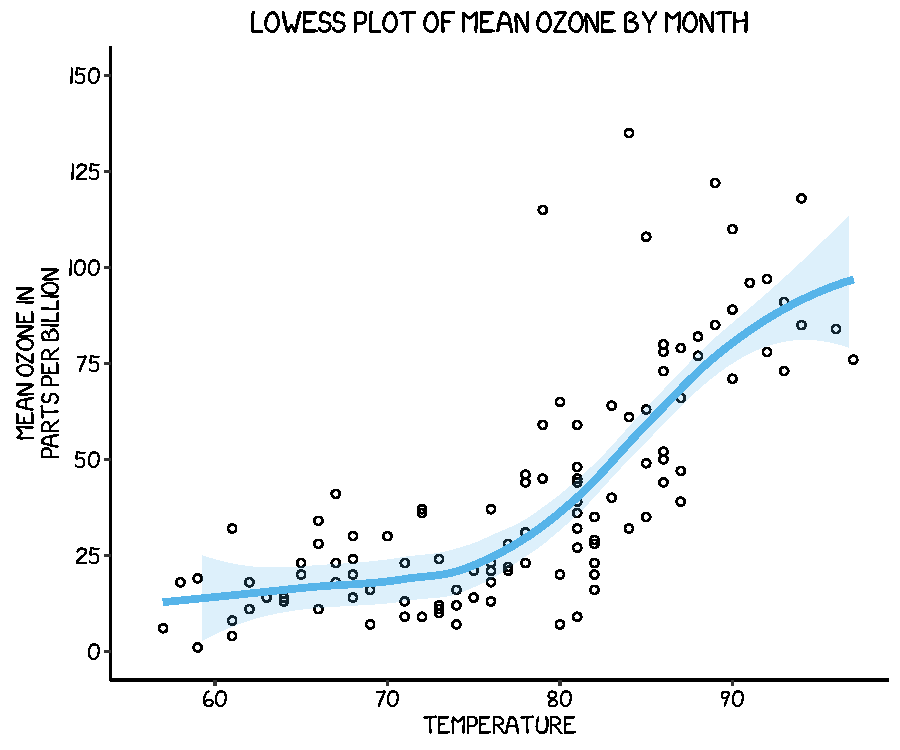
\includegraphics{12_Lowess_Plots_pdf/lowess_18-1} \end{center}

\section{\texorpdfstring{Using `The Economist'
theme}{Using The Economist theme}}\label{using-the-economist-theme}

There are a wider range of pre-built themes available as part of the
\texttt{ggthemes} package (more information on these
\href{https://cran.r-project.org/web/packages/ggthemes/vignettes/ggthemes.html}{here}).
Below we've applied \texttt{theme\_economist()}, which approximates
graphs in the Economist magazine.

\begin{Shaded}
\begin{Highlighting}[]
\NormalTok{p12 <-}\StringTok{ }\KeywordTok{ggplot}\NormalTok{(airquality, }\KeywordTok{aes}\NormalTok{(}\DataTypeTok{x =} \NormalTok{Temp, }\DataTypeTok{y =} \NormalTok{Ozone)) +}\StringTok{ }
\StringTok{  }\KeywordTok{geom_point}\NormalTok{(}\DataTypeTok{shape =} \DecValTok{21}\NormalTok{, }\DataTypeTok{colour =} \StringTok{"#1F3552"}\NormalTok{) +}\StringTok{ }
\StringTok{  }\KeywordTok{geom_smooth}\NormalTok{(}\DataTypeTok{method =} \StringTok{"loess"}\NormalTok{, }\DataTypeTok{colour =} \StringTok{"#4271AE"}\NormalTok{, }\DataTypeTok{size =} \FloatTok{1.5}\NormalTok{, }
              \DataTypeTok{alpha =} \FloatTok{0.2}\NormalTok{, }\DataTypeTok{fill =} \StringTok{"#4271AE"}\NormalTok{) +}
\StringTok{  }\KeywordTok{scale_x_continuous}\NormalTok{(}\DataTypeTok{name =} \StringTok{"Temperature"}\NormalTok{) +}
\StringTok{  }\KeywordTok{scale_y_continuous}\NormalTok{(}\DataTypeTok{name =} \StringTok{"Mean ozone in}\CharTok{\textbackslash{}n}\StringTok{parts per billion"}\NormalTok{,}
                     \DataTypeTok{breaks =} \KeywordTok{seq}\NormalTok{(}\DecValTok{0}\NormalTok{, }\DecValTok{150}\NormalTok{, }\DecValTok{25}\NormalTok{), }\DataTypeTok{limits=}\KeywordTok{c}\NormalTok{(}\DecValTok{0}\NormalTok{, }\DecValTok{150}\NormalTok{)) +}
\StringTok{  }\KeywordTok{ggtitle}\NormalTok{(}\StringTok{"LOWESS plot of mean ozone by month"}\NormalTok{) +}
\StringTok{  }\KeywordTok{theme_economist}\NormalTok{() +}\StringTok{ }\KeywordTok{scale_fill_economist}\NormalTok{() +}
\StringTok{  }\KeywordTok{theme}\NormalTok{(}\DataTypeTok{axis.line.x =} \KeywordTok{element_line}\NormalTok{(}\DataTypeTok{size=}\NormalTok{.}\DecValTok{5}\NormalTok{, }\DataTypeTok{colour =} \StringTok{"black"}\NormalTok{),}
    \DataTypeTok{axis.title =} \KeywordTok{element_text}\NormalTok{(}\DataTypeTok{size =} \DecValTok{12}\NormalTok{),}
    \DataTypeTok{legend.position=}\StringTok{"bottom"}\NormalTok{, }
    \DataTypeTok{legend.direction=}\StringTok{"horizontal"}\NormalTok{,}
    \DataTypeTok{legend.box =} \StringTok{"horizontal"}\NormalTok{, }
    \DataTypeTok{legend.text =} \KeywordTok{element_text}\NormalTok{(}\DataTypeTok{size =} \DecValTok{10}\NormalTok{),}
    \DataTypeTok{text =} \KeywordTok{element_text}\NormalTok{(}\DataTypeTok{family =} \StringTok{"OfficinaSanITC-Book"}\NormalTok{),}
    \DataTypeTok{plot.title =} \KeywordTok{element_text}\NormalTok{(}\DataTypeTok{family=}\StringTok{"OfficinaSanITC-Book"}\NormalTok{))}
\NormalTok{p12}
\end{Highlighting}
\end{Shaded}

\begin{center}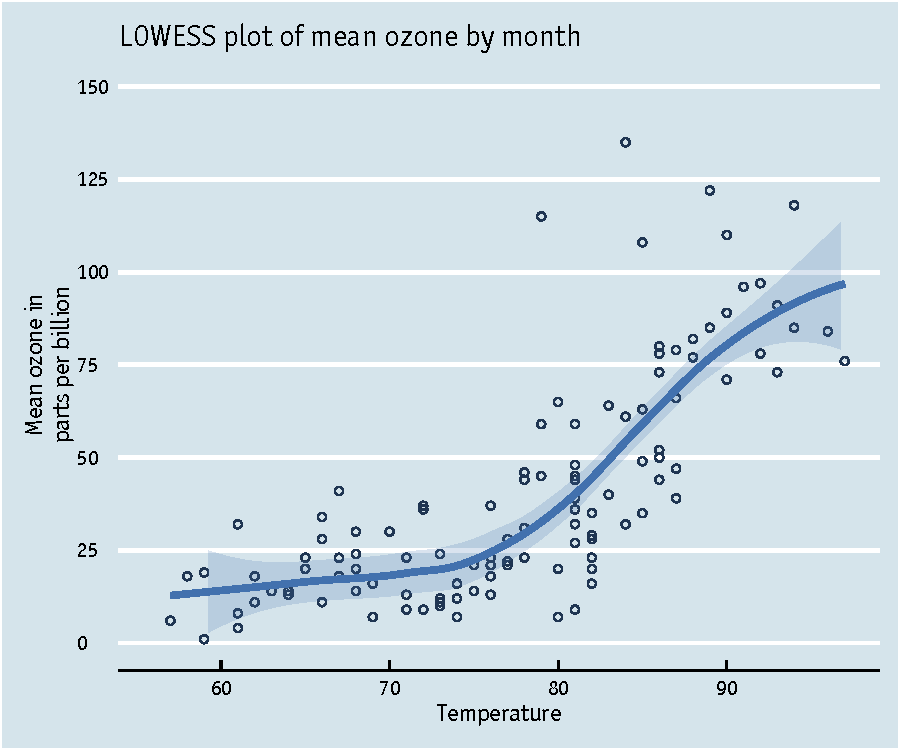
\includegraphics{12_Lowess_Plots_pdf/lowess_19-1} \end{center}

\section{\texorpdfstring{Using `Five Thirty Eight'
theme}{Using Five Thirty Eight theme}}\label{using-five-thirty-eight-theme}

Below we've applied \texttt{theme\_fivethirtyeight()}, which
approximates graphs in the nice
\href{http://fivethirtyeight.com/}{FiveThirtyEight} website. Again, it
is also important that the font change is optional and it's only to
obtain a more similar result compared to the original. For an exact
result you need `Atlas Grotesk' and `Decima Mono Pro' which are
commercial font and are available
\href{https://commercialtype.com/catalog/atlas}{here} and
\href{https://www.myfonts.com/fonts/tipografiaramis/decima-mono-pro/}{here}.

\begin{Shaded}
\begin{Highlighting}[]
\NormalTok{p12 <-}\StringTok{ }\KeywordTok{ggplot}\NormalTok{(airquality, }\KeywordTok{aes}\NormalTok{(}\DataTypeTok{x =} \NormalTok{Temp, }\DataTypeTok{y =} \NormalTok{Ozone)) +}\StringTok{ }
\StringTok{  }\KeywordTok{geom_point}\NormalTok{(}\DataTypeTok{shape =} \DecValTok{21}\NormalTok{, }\DataTypeTok{colour =} \StringTok{"red"}\NormalTok{) +}\StringTok{ }
\StringTok{  }\KeywordTok{geom_smooth}\NormalTok{(}\DataTypeTok{method =} \StringTok{"loess"}\NormalTok{, }\DataTypeTok{colour =} \StringTok{"dodgerblue"}\NormalTok{, }\DataTypeTok{size =} \FloatTok{1.5}\NormalTok{, }
              \DataTypeTok{alpha =} \FloatTok{0.2}\NormalTok{, }\DataTypeTok{fill =} \StringTok{"dodgerblue"}\NormalTok{) +}
\StringTok{  }\KeywordTok{scale_x_continuous}\NormalTok{(}\DataTypeTok{name =} \StringTok{"Temperature"}\NormalTok{) +}
\StringTok{  }\KeywordTok{scale_y_continuous}\NormalTok{(}\DataTypeTok{name =} \StringTok{"Mean ozone in}\CharTok{\textbackslash{}n}\StringTok{parts per billion"}\NormalTok{,}
                     \DataTypeTok{breaks =} \KeywordTok{seq}\NormalTok{(}\DecValTok{0}\NormalTok{, }\DecValTok{150}\NormalTok{, }\DecValTok{25}\NormalTok{), }\DataTypeTok{limits=}\KeywordTok{c}\NormalTok{(}\DecValTok{0}\NormalTok{, }\DecValTok{150}\NormalTok{)) +}
\StringTok{  }\KeywordTok{ggtitle}\NormalTok{(}\StringTok{"LOWESS plot of mean ozone by month"}\NormalTok{) +}
\StringTok{  }\KeywordTok{theme_fivethirtyeight}\NormalTok{() +}\StringTok{ }\KeywordTok{scale_fill_fivethirtyeight}\NormalTok{() +}\StringTok{   }
\StringTok{  }\KeywordTok{theme}\NormalTok{(}\DataTypeTok{axis.title =} \KeywordTok{element_text}\NormalTok{(}\DataTypeTok{family=}\StringTok{"AtlasGrotesk-Light"}\NormalTok{, }\DataTypeTok{size =} \DecValTok{12}\NormalTok{),}
    \DataTypeTok{legend.position=}\StringTok{"bottom"}\NormalTok{, }
    \DataTypeTok{legend.direction=}\StringTok{"horizontal"}\NormalTok{,}
    \DataTypeTok{legend.box =} \StringTok{"horizontal"}\NormalTok{, }
    \DataTypeTok{legend.title=}\KeywordTok{element_text}\NormalTok{(}\DataTypeTok{family=}\StringTok{"AtlasGrotesk-Light"}\NormalTok{, }\DataTypeTok{size =} \DecValTok{8}\NormalTok{),}
    \DataTypeTok{legend.text=}\KeywordTok{element_text}\NormalTok{(}\DataTypeTok{family=}\StringTok{"AtlasGrotesk-Light"}\NormalTok{, }\DataTypeTok{size =} \DecValTok{8}\NormalTok{),}
    \DataTypeTok{plot.title=}\KeywordTok{element_text}\NormalTok{(}\DataTypeTok{family=}\StringTok{"AtlasGrotesk-Medium"}\NormalTok{, }\DataTypeTok{size =} \DecValTok{16}\NormalTok{), }
    \DataTypeTok{text=}\KeywordTok{element_text}\NormalTok{(}\DataTypeTok{family=}\StringTok{"DecimaMonoPro"}\NormalTok{)) }
\NormalTok{p12}
\end{Highlighting}
\end{Shaded}

\begin{center}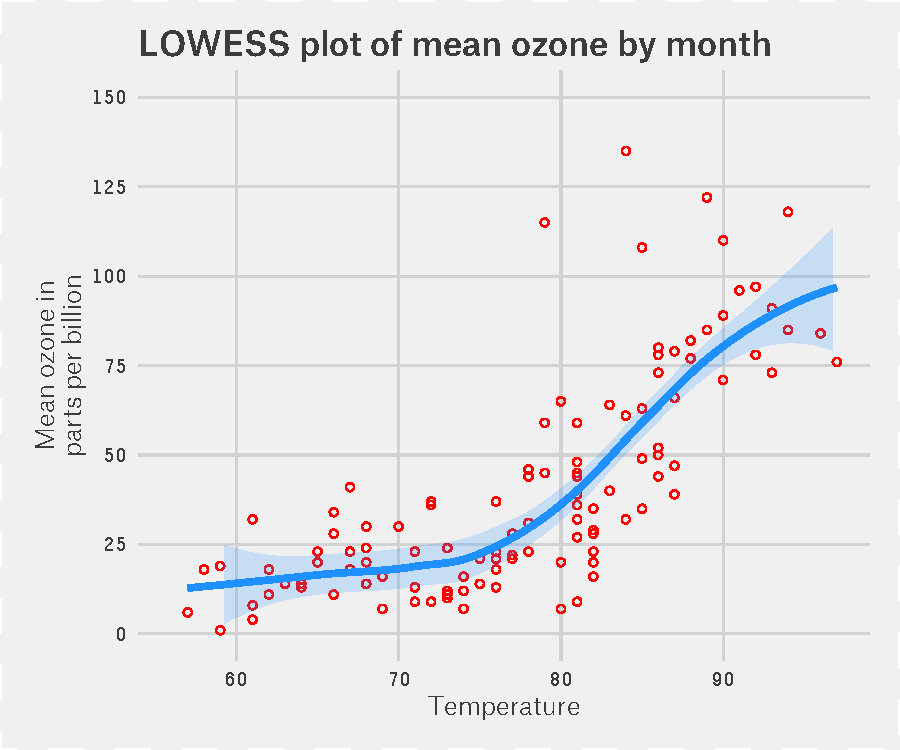
\includegraphics{12_Lowess_Plots_pdf/lowess_20-1} \end{center}

\section{Creating your own theme}\label{creating-your-own-theme}

As before, you can modify your plots a lot as \texttt{ggplot2} allows
many customisations. Here we present our original result shown at the
top of page.

\begin{Shaded}
\begin{Highlighting}[]
\NormalTok{fill <-}\StringTok{ "#4271AE"}

\NormalTok{p12 <-}\StringTok{ }\KeywordTok{ggplot}\NormalTok{(airquality, }\KeywordTok{aes}\NormalTok{(}\DataTypeTok{x =} \NormalTok{Temp, }\DataTypeTok{y =} \NormalTok{Ozone)) +}\StringTok{ }
\StringTok{  }\KeywordTok{geom_point}\NormalTok{(}\DataTypeTok{shape =} \DecValTok{21}\NormalTok{, }\DataTypeTok{colour =} \StringTok{"darkblue"}\NormalTok{) +}\StringTok{ }
\StringTok{  }\KeywordTok{geom_smooth}\NormalTok{(}\DataTypeTok{method =} \StringTok{"loess"}\NormalTok{, }\DataTypeTok{colour =} \NormalTok{fill, }\DataTypeTok{size =} \FloatTok{1.5}\NormalTok{, }
              \DataTypeTok{alpha =} \FloatTok{0.2}\NormalTok{, }\DataTypeTok{fill =} \NormalTok{fill) +}
\StringTok{  }\KeywordTok{scale_x_continuous}\NormalTok{(}\DataTypeTok{name =} \StringTok{"Temperature"}\NormalTok{) +}
\StringTok{  }\KeywordTok{scale_y_continuous}\NormalTok{(}\DataTypeTok{name =} \StringTok{"Mean ozone in}\CharTok{\textbackslash{}n}\StringTok{parts per billion"}\NormalTok{,}
                     \DataTypeTok{breaks =} \KeywordTok{seq}\NormalTok{(}\DecValTok{0}\NormalTok{, }\DecValTok{150}\NormalTok{, }\DecValTok{25}\NormalTok{), }\DataTypeTok{limits=}\KeywordTok{c}\NormalTok{(}\DecValTok{0}\NormalTok{, }\DecValTok{150}\NormalTok{)) +}
\StringTok{  }\KeywordTok{ggtitle}\NormalTok{(}\StringTok{"LOWESS plot of mean ozone by month"}\NormalTok{) +}
\StringTok{  }\KeywordTok{theme_bw}\NormalTok{() +}
\StringTok{  }\KeywordTok{theme}\NormalTok{(}\DataTypeTok{panel.border =} \KeywordTok{element_rect}\NormalTok{(}\DataTypeTok{colour =} \StringTok{"black"}\NormalTok{, }\DataTypeTok{fill=}\OtherTok{NA}\NormalTok{, }\DataTypeTok{size=}\NormalTok{.}\DecValTok{5}\NormalTok{),}
    \DataTypeTok{panel.grid.major =} \KeywordTok{element_line}\NormalTok{(}\DataTypeTok{colour =} \StringTok{"#d3d3d3"}\NormalTok{), }
    \DataTypeTok{panel.grid.minor =} \KeywordTok{element_blank}\NormalTok{(), }
    \DataTypeTok{panel.border =} \KeywordTok{element_blank}\NormalTok{(), }\DataTypeTok{panel.background =} \KeywordTok{element_blank}\NormalTok{(),}
    \DataTypeTok{plot.title =} \KeywordTok{element_text}\NormalTok{(}\DataTypeTok{size =} \DecValTok{13}\NormalTok{, }\DataTypeTok{family =} \StringTok{"Tahoma"}\NormalTok{, }\DataTypeTok{face =} \StringTok{"bold"}\NormalTok{),}
    \DataTypeTok{text=}\KeywordTok{element_text}\NormalTok{(}\DataTypeTok{family =} \StringTok{"Tahoma"}\NormalTok{), }
    \DataTypeTok{axis.title =} \KeywordTok{element_text}\NormalTok{(}\DataTypeTok{face=}\StringTok{"bold"}\NormalTok{, }\DataTypeTok{size =} \DecValTok{10}\NormalTok{),}
    \DataTypeTok{axis.text.x =} \KeywordTok{element_text}\NormalTok{(}\DataTypeTok{colour=}\StringTok{"black"}\NormalTok{, }\DataTypeTok{size =} \DecValTok{8}\NormalTok{),}
    \DataTypeTok{axis.text.y =} \KeywordTok{element_text}\NormalTok{(}\DataTypeTok{colour=}\StringTok{"black"}\NormalTok{, }\DataTypeTok{size =} \DecValTok{8}\NormalTok{)) }
\NormalTok{p12}
\end{Highlighting}
\end{Shaded}

\begin{center}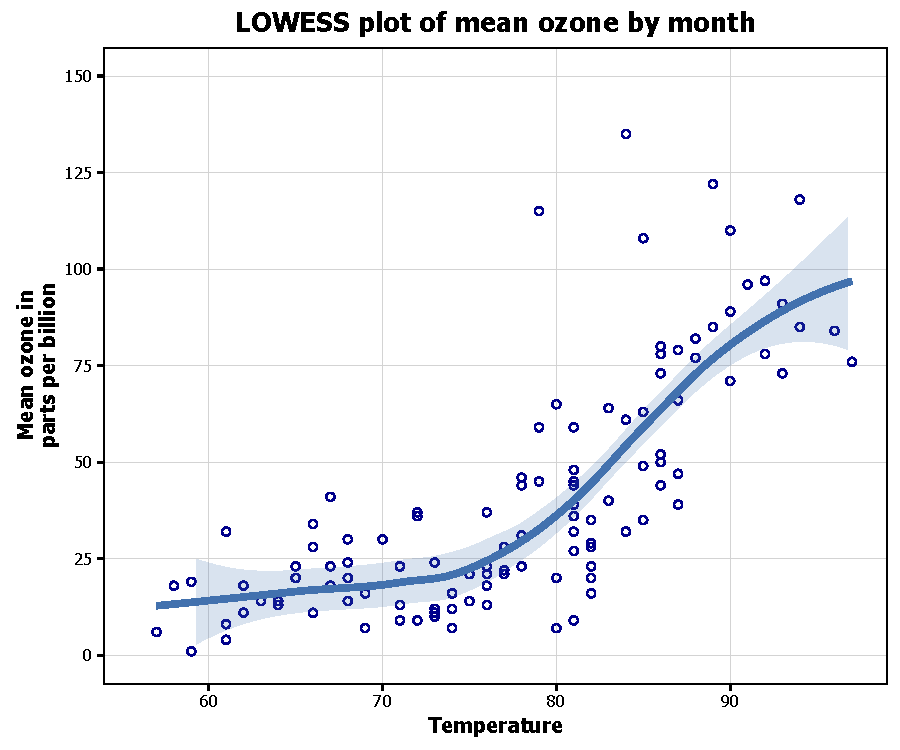
\includegraphics{12_Lowess_Plots_pdf/lowess_21-1} \end{center}

\end{document}
